\documentclass[12pt,twoside,final]{book}
\usepackage{natbib}

%\usepackage[portuges,brazil]{babel}
\usepackage[latin1]{inputenc}
\usepackage{hyperref}
\usepackage{enumerate}

\usepackage{indentfirst}
\usepackage{ae}
%\usepackage{harvard}
\usepackage{amssymb,fancyhdr,fancybox,epsfig,psfrag,amsmath,tabularx}
\usepackage[paperwidth=8.5in,paperheight=11in,hmargin={25mm,20mm},vmargin={20mm,20mm}]{geometry} %tamanho letter

%Packages added by me
\usepackage{appendix}
\usepackage{multirow}


\usepackage[color]{showkeys}
\definecolor{refkey}{rgb}{0.39,0.58,1}
\definecolor{labeled}{rgb}{1,0,0}
\usepackage[Lenny]{fncychap}
\setlength{\headheight}{15pt}

%=========================================== Headers =========================================

\renewcommand{\chaptermark}[1]{\markboth{\chaptername\ \thechapter. \ #1}{ }}
\renewcommand{\sectionmark}[1]{\markright{\thesection. \ #1}}
\fancyhead{}
\fancyfoot{}
\fancyhead[LE,RO]{\thepage}
\fancyhead[RE]{\nouppercase{\leftmark}}
\fancyhead[LO]{\nouppercase{\rightmark}}
%==============================================================================================


% Espacos H2, Hoo, L2, Loo
\newcommand\Hi{{\mathcal{H}}_{\infty}}
\newcommand\Hd{{\mathcal{H}}_{2}}
\newcommand\Li{{\mathcal{L}}_{\infty}}
\newcommand\Ld{{\mathcal{L}}_{2}}


\def\reais{{\rm I\kern-.17em R}} % R de reais
\def\Dest{{\rm I\kern-.17em D}} % R de reais
\newcommand{\Dgest}{\ensuremath{\mathcal{D}}}
\newcommand{\naturais}{\mathbb{N}}
\newcommand{\inteiros}{\mathbb{Z}_{+}}
\newcommand{\matlab}{{\sc Matlab}}

%super parenteses
\makeatletter
\def\Biggg#1{{\hbox{$\left#1\vbox to29\p@{}\right.\n@space$}}}
\newdimen\bracketwidth
\settowidth{\bracketwidth}{\Biggg(} \makeatother


%\newcommand{\carinha}{\raisebox{-.2ex}{\epsfxsize 3mm \epsffile{cara.eps}}}

% Bolds
\newcommand{\I}{{\bf I}}
\newcommand{\Z}{{\bf 0}}
\newcommand{\Bfres}{\mathcal{B}}

% funcoes
\newcommand{\Tr}{\mbox{Tr}}

% Referencia com parenteses
\newcommand{\bref}[1]{\mbox{(\ref{#1})}}

% Ambiente de equacoes
\newcommand\be{\begin{equation}}
\newcommand\ee{\end{equation}}
\newcommand\vi{\vspace{\baselineskip}}

% newtheorems e similares

\newtheorem{teorema}{\noindent{\bf Teorema} }[chapter]
\newtheorem{lema}{\noindent{\bf Lema} }[chapter]
\newtheorem{corolario}{\noindent{\bf Corol�rio} }[chapter]
\newenvironment{prova}{\noindent{\bf Prova:}}{\null\hfill $\rule{1.5mm}{1.5mm}$}
\newtheorem{definicao}{\noindent{\bf Defini��o} }[chapter]

\newcommand{\simplex}{\Delta_N}



\newcommand{\Aal}{A(\alpha)}
\newcommand{\Bal}{B(\alpha)}
\newcommand{\Cal}{C(\alpha)}
\newcommand{\Dal}{D(\alpha)}


\newcommand{\Pal}{P(\alpha)}
\newcommand{\Gal}{G(\alpha)}
\newcommand{\Hal}{H(\alpha)}
\newcommand{\Qal}{Q(\alpha)}
\newcommand{\Xal}{X(\alpha)}
\newcommand{\Xual}{X_1(\alpha)}
\newcommand{\Xdal}{X_2(\alpha)}

\newcommand{\Sfr}{\mathcal{S}}

\newcommand{\Xfal}{\mathcal{X}(\alpha)}
\newcommand{\Bfal}{\mathcal{B}(\alpha)}
\newcommand{\Qfal}{\mathcal{Q}(\alpha)}
\newcommand{\Sfal}{\mathcal{S}(\alpha)}

\newcommand{\Kfr}{\mathcal{K}}
\newcommand{\Ifr}{\mathcal{I}}
\newcommand{\Afr}{\mathcal{A}}
\newcommand{\Pfr}{\mathcal{P}}
\newcommand{\Cfr}{\mathcal{C}}
\newcommand{\Gfr}{\mathcal{G}}


\begin{document}

\pagenumbering{roman}
\pagestyle{plain}

%Tese em portugu�s
%================================================================================================
%================================= PRIMEIRA FOLHA INTERNA  ======================================
%================================================================================================

\thispagestyle{empty} %Tirando o numero da primeira p�gina
\vspace*{2.0cm}
\begin{center}
\large Tiago de Freitas Pereira
\end{center}

\vspace*{6.8cm}

\begin{center}
{\sc A Comparative Study of Countermeasures to Detect Spoofing Attacks in Face Authentication Systems}
\end{center}

\vspace*{3.25cm}


\null \vfill

\begin{center}
Campinas\\2013
\end{center}
\newpage
% parte de tr�s da primeira folha interna fica em branco

\null \vfill
\newpage

%================================================================================================
%====================================== FOLHA DE ROSTO ==========================================
%================================================================================================
\begin{center}
\large Universidade Estadual de Campinas\\
Faculdade de Engenharia El�trica e de Computa��o
\end{center}

\vspace*{1.5cm}
\begin{center}
\large Tiago de Freitas Pereira
\end{center}


\vspace*{2.3cm}

\begin{center}
{\sc A Comparative Study of Countermeasures to Detect Spoofing Attacks in Face Authentication Systems}

\end{center}

\vspace*{3.0cm}

\begin{flushright}
\begin{minipage}{9.0cm}
Disserta��o de Mestrado apresentada na Faculdade de Engenharia El�trica e de Computa��o como  parte dos
requisitos exigidos para a obten��o do t�tulo de Mestre em Engenharia El�trica. �rea de
concentra��o: Computa��o

\vspace*{0.5cm}
Orientador: Professor Doutor Jos� Mario De Martino

\end{minipage}
\end{flushright}

\null \vfill
\begin{minipage}{7cm}
\small
Este exemplar corresponde a vers�o final da disserta��o de mestrado apresentado pelo
aluno, e orientado pelo Prof. Dr. Jos� Mario De Martino\\[4mm]
\rule{7.0cm}{0.2mm} \hfill
\end{minipage}

\vspace*{0.5cm}

\begin{center}
Campinas\\2013
\end{center}

\newpage
\null \vfill
\newpage

%Tese em portugu�s e ingl�s
%%================================================================================================
%================================= PRIMEIRA FOLHA INTERNA  ======================================
%================================================================================================
\vspace*{2.0cm}
\begin{center}
\large Fulano de Tal
\end{center}


\vspace*{4.8cm}

\begin{center}
{\sc \Large  Coloque aqui o t�tulo da tese; Coloque aqui o t�tulo \\ da tese;
Coloque aqui o t�tulo da tese;  Coloque aqui }
\end{center}

\vspace*{1cm}
\begin{center}
{\sc \Large  Place here the thesis' title;Place here the thesis'\\ title; Place here the thesis' title ;
Place here }
\end{center}

\vspace*{3.25cm}


\null \vfill

\begin{center}
Campinas\\2012
\end{center}
\newpage
% parte de tr�s da primeira folha interna fica em branco

\null \vfill
\newpage


%================================================================================================
%====================================== FOLHA DE ROSTO ==========================================
%================================================================================================

\begin{center}
\large Universidade Estadual de Campinas\\
Faculdade de Engenharia El�trica e de Computa��o
\end{center}

\vspace*{1.0cm}
\begin{center}
\large Fulano de Tal
\end{center}


\vspace*{1.3cm}

\begin{center}
{\sc  Coloque aqui o t�tulo da tese; Coloque aqui o t�tulo da tese;  \\ 
Coloque aqui o t�tulo da tese;  Coloque aqui o t�tulo da tese;}
\end{center}

\vspace*{0.5cm}

\begin{center}
{\sc   Place here the thesis' title;Place here the thesis'\\ title; Place here the thesis' title ;
Place here }
\end{center}

\vspace*{1.0cm}

\begin{flushright}
\begin{minipage}{11.0cm}
Tese de doutorado apresentada � Faculdade de Engenharia El�trica e de Computa��o como  parte dos
requisitos exigidos para a obten��o do t�tulo de Doutor em Engenharia El�trica. �rea de
concentra��o: Automa��o. 

\vspace*{0.5cm}

Doctorate thesis presented to the School of Electrical and Computer Engineering
in partial fulfillment of the requirements for the degree of Doctor in Electrical
Engineering. Concentration area: Automation

\vspace*{1.0cm}
Orientador (Tutor): Prof. Dr. Pedro Luis Dias Peres

\end{minipage}
\end{flushright}

\null \vfill
\begin{minipage}{7cm}
\small
Este exemplar corresponde � vers�o final da tese defendida pelo
aluno, e orientada pelo Prof. Dr. Pedro Luis Dias Peres\\[4mm]
\rule{7.0cm}{0.2mm} \hfill 
\end{minipage}

\begin{center}
Campinas\\2012
\end{center}

%================================================================================================
%============================== Ficha (Somente na vers�o final) =================================
%================================================================================================
\newpage

\begin{center}
\vspace*{10cm}
Insira nesta p�gina a sua ficha catalogr�fica (somente vers�o final). Obs. � conveniente
converter o documento fornecido pela BAE (normalmente .doc) em um arquivo .ps. Para a vers�o
preliminar da tese (antes da defesa), simplesmente remova essa p�gina.
\end{center}
% Observa��o: a ficha fornecida pela BAE normalmente � fornecida em formato .doc. Existem diversas
% maneiras de converter .doc em .ps. 

% Descomente as duas pr�ximas linhas (e comente acima desde o begin{center} at� o end{center}) para inserir a ficha catalogr�fica caso a mesma j�  tenha sido convertida para .ps (no caso ficha.ps)

%\epsfxsize=0.925\columnwidth
%\epsffile{ficha.ps}

\null \vfill
\newpage

%================================================================================================
%============================== Folha de aprova��o (Somente na vers�o final) ====================
%================================================================================================


\begin{center}
\vspace*{10cm}
Insira nesta p�gina a folha de aprova��o fornecida pelo seu programa de p�s-gradua��o (somente vers�o final). 
Obs. � conveniente scanear o documento e convert�-lo para o formato .ps. Para a vers�o
preliminar da tese (antes da defesa), simplesmente remova essa p�gina.
\end{center}

% Escanear a folha de aprova��o fornecida pela CPG e converter para .ps ou .eps. A id�ia
% � inserir como uma figura. � muito prov�vel que ser� necess�rio fazer ajustes no
% tamanho, mexendo no comando \epsfxsize

% Descomente as duas pr�ximas linhas (e comente acima desde o \begin{center} at� o \end{center})
%\epsfxsize=0.985\columnwidth
%\hspace*{-1.25cm}\epsffile{aprov.eps}

\null \vfill
\newpage
% verso da folha de aprova��o em branco
\null \vfill
\newpage


%======================================== Dedicat�ria =========================================
\null\vfill
\begin{flushright}
\begin{minipage}{6.5cm}
{\sc Dedicat�ria}
\end{minipage} \\[8mm]
\end{flushright}
\newpage %verso em branco

\null
%==============================================================================================


%======================================= Agradecimentos =======================================
\chapter*{Acknowledgment}

%\noindent Text \\[2mm]

\noindent More than two years were necessary to finish this work and many people got involved. \\

First of all I would like to thank Prof. Dr. Jos\'e Mario De Martino for his guidance and patience in this journey. \\

Many thanks to Dr. S\'ebastien Marcel, Dr. Andr\'e Anjos and Ivana Chingovska from the IDIAP Research Institute. Their supervision in the four months that I spend in Switzerland was definitely decisive to complete this masters dissertation. A special thanks to Dr. Andr\'e Anjos for his guidance, friendship and the doses of cacha\c{c}a. I also would like to thank Dr. Manuel G{\"u}nter, Dr. Elie El Khoury, Dr. Nesli Erdogmus, Laurent El Shafey and Jukka Komulainen (University of Oulu) for their support and companionship. \\

Thanks to CPqD, for encourage me in this project releasing so many hours of work. A special thanks to Norberto Alves Pereira, Claudinei Martins, Eliana De Martino, Emilio Nakamura, Marcus de Assis Angeloni, Jos\'e Eduardo de Carvalho Silva, Ricardo Violatto, Mario Uliani and the big master Flavio Sim\~oes. \\

To my friends Geovane Shimizu, Marcus Angeloni, Bruno Cafeo and Diego Silva for just being there. \\

To my parents Antonio Alberto (Tote) and Sueli, and brother Rodrigo for the unconditional love and support, even don't understanding a bit what I am doing. A special thanks to my grandma Christina. She was a great example of a teacher and also my first one. \\

A very special thanks to my best friend and fianc\'ee Carolina Scarton, for her support and unconditional love during these years.


\newpage %verso em branco

\null

%==============================================================================================


%======================================== Frase Miss Brasil ===================================
\newpage
\null\vfill
\begin{flushright}
\begin{minipage}{9.0cm}
A maravilhosa disposi��o e harmonia do universo s� pode ter tido origem segundo o plano de um Ser
que tudo sabe e tudo pode. Isto fica sendo a minha �ltima e mais elevada descoberta.
\end{minipage}
\end{flushright}


\begin{flushright}
 Isaac Newton
\end{flushright}

\newpage %verso em branco

\null
%==============================================================================================



\baselineskip 1.1 \baselineskip

%================================= Resumo e Abstract ========================================
\chapter*{Resumo}


\begin{quotation}
\noindent Autentica��o de usu�rios � uma tarefa crucial para proteger informa��es e nesta �rea a biometria de face apresenta algumas vantagens. A biometria de face � natural, f�cil de interagir e � uma das biometrias que possui um processo de coleta menos invasiva. Trabalhos recentes tem revelado que a biometria de face � vulner�vel a ataques de \textit{spoofing} utilizando equipamentos baratos. Contramedidas tem sido propostas para mitigar este tipo de vulnerabilidade. Por�m uma boa parte das contramedidas apresentadas na literatura s�o avaliadas utilizando m�tricas distintas e muitas vezes em bases de dados privadas impossibilitando uma compara��o justa das mesmas. Este projeto tem como objetivo apresentar um estudo comparativo de contramedidas contra ataques de \textit{spoofing} em sistemas de autentica��o facial.


\vspace*{0.5cm}

\noindent Palavras-chave:  Antispoofing, Detec��o de vitalidade, Contramedidas, Reconhecimento Facial, Biometria
\end{quotation}


\newpage
\null



\chapter*{Abstract}


\begin{quotation}


\noindent User authentication is an important step to protect information and in this field face biometrics is advantageous. Face biometrics is natural, easy to use and less human-invasive. Unfortunately, recent work has revealed that face biometrics is vulnerable to spoofing attacks using low-tech equipments. Countermeasures have been proposed in order to mitigate this vulnerabilities. However several works in the literature present evaluations using different metrics and in private database making the comparison of countermeasures a difficult task. The main goal of this masters project is to provide a comparative study of countermeasures against \textit{spoofing} attacks.


\vspace*{0.5cm}

\noindent Key-words:  Antispoofing, Liveness detection, Countermeasure, Face Recognition, Biometrics
\newpage% verso em branco
\end{quotation}

\newpage
\null




%=============================== lista de tabelas e figuras ==========================
\listoffigures
\newpage


\listoftables
\newpage



%============================ acr�nimos, s�mbolos e nota��es ========================
%============================Acronimos e Nota��o =================================================

\chapter*{Lista de Acr�nimos e Nota��o}

\begin{tabular}{ll}
LMI  & Linear Matrix Inequality (desigualdade matricial linear)\\
LFT  & Linear Fractional Transformation (transforma��o linear fracion�ria)\\
LPV  & Linear Parameter-Varying (linear com par�metros variantes)\\
IQC  & Integral Quadratic Constraint (restri��o de integral quadr�tica)\\
\end{tabular}

\vspace*{1cm}

\begin{tabular}{ll}
$\star$ & indica bloco sim�trico nas LMIs\\
$L > 0$ & indica que a matriz $L$ � sim�trica definida positiva\\
$L \geq 0$ & indica que a matriz $L$ � sim�trica semi-definida positiva\\
$A$ & nota��o para matrizes (letras mai�sculas do alfabeto latino)\\
$A'$ & ($'$), p�s-posto a um vetor ou matriz, indica a opera��o de transposi��o\\
$\reais$ & conjunto dos n�meros reais\\
$\mathbb{Z}$ & conjunto dos n�meros inteiros\\
$\mathbb{Z}_+$ & conjunto dos n�meros inteiros n�o negativos\\
$\mathbb{N}$ & conjunto dos n�meros naturais (incluindo o zero)\\
$\I$ & matriz identidade de dimens�o apropriada\\
$\Z$ & matriz de zeros de dimens�o apropriada\\
$g!$ & s�mbolo (!), denota fatorial, isto �, $g!=g (g-1) \cdots (2) (1)$ para $g \in \mathbb{N}$\\
$N$ & especialmente utilizada para denotar o n�mero de v�rtices de um politopo\\
$n$ & especialmente utilizada para representar a ordem uma matriz quadrada\\
$\simplex$ & simplex unit�rio de $N$ vari�veis\\
$\alpha$ & especialmente utilizada para representar as incertezas de um sistema
\end{tabular}

\newpage
% verso em branco (sem numera��o na p�gina).


%==============================================================================================


%=============================== sum�rio =============================================
\tableofcontents


\newpage
%caso o sum�rio acabe em uma p�gina �mpar, o verso ser� em branco
\null \vfill
\newpage

%Agora muda para o estilo fancy
\pagestyle{fancy}

%%%%%%
% CRIAR FINAL REMARKS
%%%%%%%%
\pagenumbering{arabic}

\chapter{Introduction}
\label{chap:introduction}

In a modern society, the authentication procedure is an important task to protect data and resources (physical or digital). Consisting of a confirmation of a claimed identity, the authentication procedure is the first and most critical task of security step, restricting access to unauthorized users. 

Biometrics is the science of recognizing the identity of a person based on their physical attributes and / or behavior, such as face, fingerprints, hand veins, voice or iris \cite{li2011handbook}. The use of biometrics in an authentication procedure has some advantages. Naturally, is not possible to forget or transfer a biometric trait and it hardly disappears (perhaps only in case of a seriously accidents). However, biometrics has some drawbacks. Compared with regular authentication systems, such as passwords or tokens, which are precise, biometric authentication systems have probabilistic behavior. It turns out that biometrics hardly has perfect match; therefore, authentication systems have to deal with error rates. These errors rates can vary depending on a number of factors. As an example, our voice can vary drastically  when we get sick or when we are under stress and this impacts a speaker authentication system. Aging, illumination, pose and face expressions are classical issues in face authentication systems.


The use of biometrics in our daily lives has grown in the last decade and we can quote several examples of this. The confirmation of an identity in the brazilian electoral process is based on fingerprints. In Brazil, a bank replaced the use of passwords to palm vein authentication in ATMs. The demand for security pushes the market to biometrics. A recent marked research estimates that the overall market for voice and face biometrics is expected to reach nearly US\$3 billions by the end of 2018\footnote{\url{http://www.biometricupdate.com/201307/voice-biometrics-and-how-far-weve-come/?goback=\%2Egde\_40210\_member\_258411747}}.


A biometric authentication system can be represented with the simple flow chart in Figure \ref{fig:diagram_attacks}.

\begin{figure}[!htb]
\begin{center}
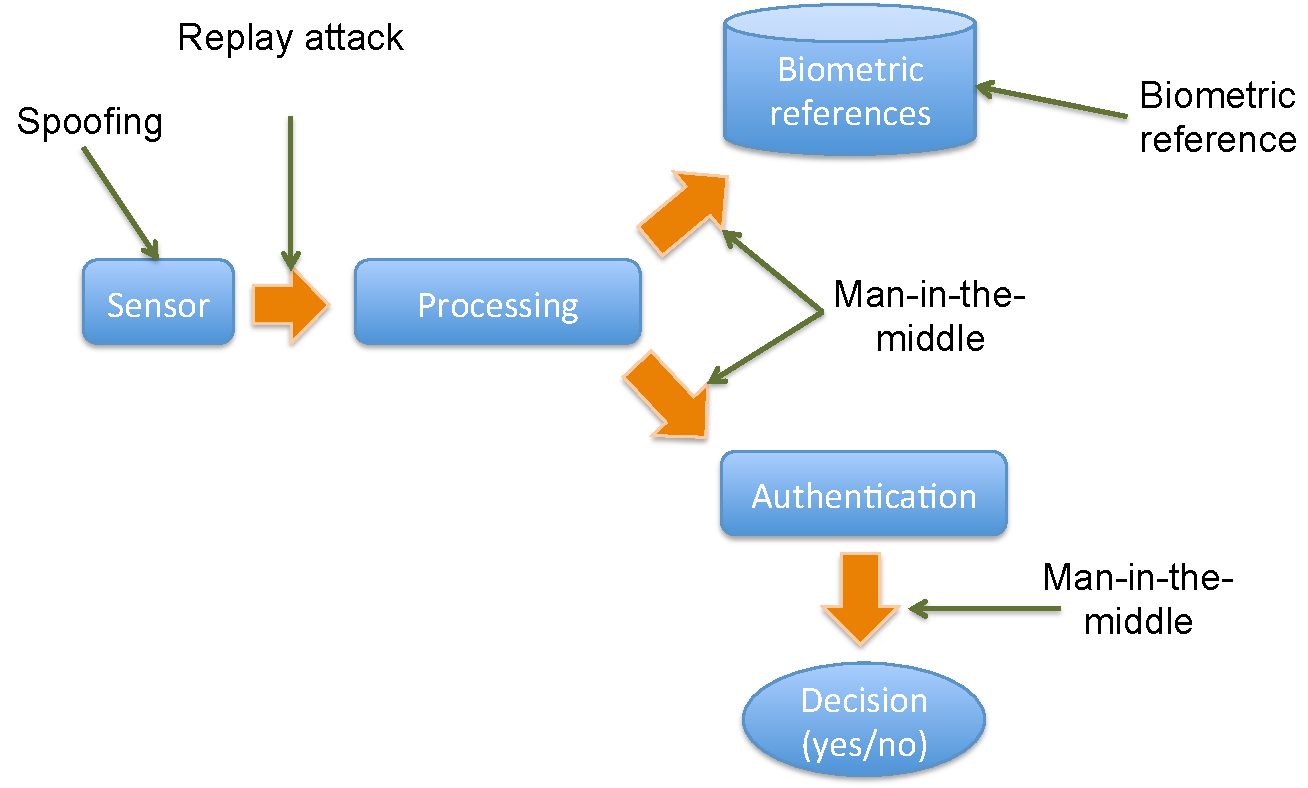
\includegraphics [width=14cm] {images/diagram_attacks.pdf}
\caption[Simple architecture of a regular biometric authentication system]{Simple architecture of a regular biometric authentication system (adapted from \cite{xiao2005security})} \label{fig:diagram_attacks}
\end{center}
\end{figure}

Firstly, the biometric trait is captured using a some kind of sensor. Secondly, the captured biometric trait is processed in order to extract the biometric features. When it is in an enrollment procedure, these features will generate a biometric reference, and it will be stored in a database. In an authentication procedure, these features will be compared with the stored biometric reference. It is possible to observe, in the same Figure, that attacks can be done at any point of the architecture \cite{xiao2005security}. 
%The next subsections discuss each one of the possible points of attack and how to mitigate it.

%\subsection{Replay attack}
%\label{sec:rep}

The \textbf{replay attack} is performed by injecting a biometric data previously sent, of the target identity, in order to have a non authorized access. This data can be obtained sniffing the biometric authentication software. To mitigate this kind of attack, the biometric system should ensure that the provided data was not injected artificially \cite{xiao2005security}. A common way to protect against this kind of attack, is to associate a timestamp to the data. As it is improbable to have exactly the same biometric data in different times, this method can be quite effective.

%\subsection{Biometric reference attack}

The \textbf{biometric reference attack} is performed where the biometrics are stored. This kind of attack, include actions such as the inclusion, removing, modifying and steal biometric references. Among this actions, the possibility to steal a biometric reference is the most dangerous threat, since it is possible to work in a reverse engineering process to regenerate the biometric trait. 

Using a hill climbing technique to optimize to the position and the orientation of the minutia \cite{MartinezDiaz2006} and \cite{hill2001risk} shown that is possible to generate synthetic fingerprints compatible with fingerprints stored in a database. Fake fingers (with a real fingerprint) with gummy or silicone can be generated with this minutia. It is possible also to inject these minutia in the \textbf{Processing} module (see Figure \ref{fig:diagram_attacks}) in order to deceive the authentication system. 

To mitigate the risk of this kind of attack, best practices in security recommends to encrypt the biometric references and to increase the policy to access these biometric references. 

%\subsection{Man-in-the-middle}

In the \textbf{man in the middle attack}, the biometric data is intercepted in any point of the architecture in Figure \ref{fig:diagram_attacks}.  As shown in the Figure \ref{fig:diagram_attacks}, the attacker can:
\begin{itemize}
        \item Manipulate the matching score;
        \item Manipulate the biometric authentication response;
        \item Steal biometric data;
        \item Inject biometric data (as shown in the replay attack).
\end{itemize}

The same security recommendations aforementioned to deal with this security breaks can be used here; i.e. encrypt the data before transmission, increase the security grants and so on. 

%\subsection{Ataque de Spoofing}

The \textbf{spoofing attack}, in biometric systems, is a direct attack to the biometric sensor; i.e. a forged biometric trait is presented to the biometric sensor in order to deceived it. The goal is to pretend to be someone else in order to get forbidden privileges. Most of biometric systems can be spoofed. Next subsections presents a brief discussion about spoofing in different biometric traits:

\subsubsection{Fingerprint}

In fingerprints verification systems, the attacker can forge a fingerprint with different materials (gummy, silicone, etc). \cite{matsumoto2002impact} and \cite{leyden2002gummi} discusses how to generate fake fingerprints using materials easily found in supermarkets. Figure \ref{fig:finger_attack} shows how easy is to create a molds from a live fingers and to reproduce its fingerprints with gummy. This fake fingers can be used  to spoof a fingerprint biometric systems.

\begin{figure}[!htb]
\begin{center}
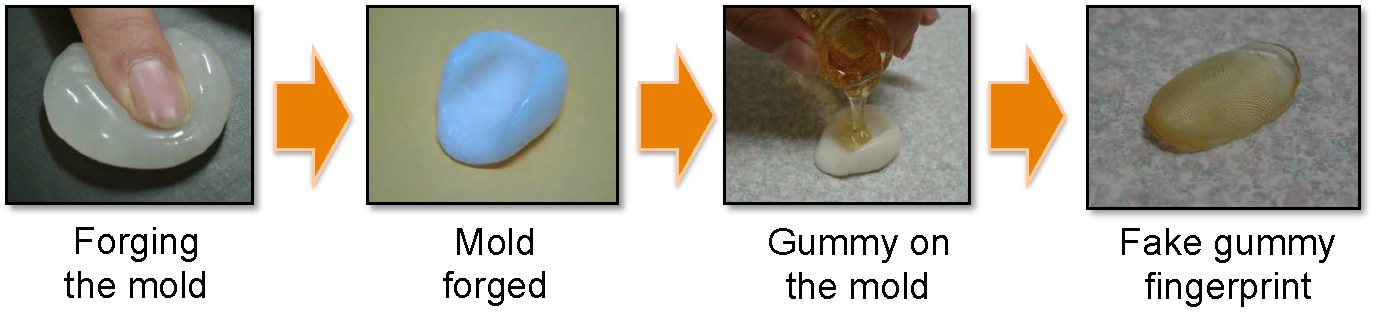
\includegraphics [width=16cm] {images/finger_print_attack.pdf}
\caption[Creating a fake fingerprint]{Creating a fake fingerprint (Adapted from \cite{matsumoto2002impact})} \label{fig:finger_attack}
\end{center}
\end{figure}

Recently in Brazil (2013), was reported that doctors in S\~ao Paulo were arrested after being caught in the act of using fake fingers made of silicone and imprinted with real fingerprints to defraud a hospital's biometric punch-in clock\footnote{\url{http://www.foxnews.com/us/2013/03/13/brazilian-doctors-use-fake-silicone-fingers-to-defraud-hospital-punch-in-clock/}}.

A more sophisticated attack is discussed in \cite{MartinezDiaz2006} and \cite{hill2001risk}. These papers use a hill climbing technique to optimize  the position and the orientation of the minutia. With this optimization was possible to generate fingerprints compatible for match.

%Using a hill climbing technique to optimize to the position and the orientation of the minutia  shown that is possible to generate fingerprints compatible with fingerpri
%A more sophisticated attack were discussed in \cite{uludag2004attacks}. This paper uses a hill climbing procedure to optimize the position and the orientation of the minutia in a minutia based fingerprint verification system. The optimized result of the minutia can be used to generate a fake finger.

%FALAR DOS SENSORES.

%http://www.tabularasa-euproject.org/news/selected-news-related-to-spoofing-attacks

\subsubsection{Speaker}

For speech biometrics, the attacker can forge a human voice by mimicry or recording the voice of the target identity and replaying back to the microphone. 

\cite{chetty2004liveness} and \cite{eveno2005speaker} address the problem using audio-visual features. The first one proposes a bi-modal authentication system using the face information in order to increase security. The second one correlates the lip movements with the content of the speech as a security barrier.

\cite{QimingZhu} analyse the speech signal itself applying the 1-dimensional $LBP$ (Local Binary Pattern) followed by a SVM (Support Vector Machines) in order to detect spoofs.

\subsubsection{Iris}

Iris biometrics has been traditionally regarded as one of the most reliable and accurate biometric traits, but as the other biometric traits it can also be spoofed. A simple way to spoof an iris recognition system is using a high quality printed image. More sophisticated attacks using contact lenses can also be carried out.

Countermeasures to deal with this kind of attacks can be deployed in hardware (with a specific equipment) or in the software \cite{Galbally_ICB-2012}. Especially in the software level, \cite{Galbally_ICB-2012} addresses the problem using various type of features, including a set of  high pass filters, motion features and occlusion filters in the iris images followed by a binary classifier as countermeasure. 

An approach based on textures was carried out by \cite{ZhuoshiWei}. This countermeasure uses the co-occurrence matrix descriptor followed by a binary classifier.

%Measuring the pupil reflex using a set of high filters, \cite{kanematsu2007highly}
% \cite{johnson2010multimodal}, \cite{kanematsu2007highly} and \cite{pacut2006aliveness} are works addressing spoofing attacks in iris biometric system. 

\subsubsection{Face}

Recently, the media has reported some situations of attacks in deployed face recognition systems. Using simple photographs, a research group from University of Hanoi showed how easy is to spoof the face authentication systems deployed in Lenovo, Asus and Toshiba Laptops \cite{BlackHat2009}. Since the release \textit{Ice Cream Sandwich}, the Android OS come with a built-in face authentication system to unlock the mobile phone. Since then, it has been extensively demonstrated around the web how easy it is to spoof this face recognition system\footnote{\url{http://www.itproportal.com/2011/11/14/ice-cream-sandwich-facial-recognition-cracked/}}. As a consequence, an eye blinking detection has been introduced in the most recent version of the Android OS. Spoofing in face authentication will be discussed in details in the Chapter \ref{chap:Spoofing}. \\ \\ 

Several technologies related to information security can be deployed in a biometric authentication systems in order to mitigate the mentioned attacks. We can highlight:
\begin{itemize}
        \item Encrypt the biometric data;
        \item Improve the security policies;
        \item Convey the biometric data using a secure channel;
        \item Deploy all modules of the architecture in a physical arrangement that cannot be penetrated;
        \item Using more than one authentication factor.
\end{itemize}
However, in a spoofing attack, the target is the biometric sensor, and in the architecture presented in Figure \ref{fig:diagram_attacks}, is not possible to apply any of the security tools to prevent this kind of attack, becoming the most fragile point. To mitigate this kind of vulnerability, effective countermeasures against face spoofing have to be deployed.


\section{Scope and Contributions}
\label{sec:scope}

Focusing in antispoofing countermeasures for face authentication, the goal of this masters dissertation is two fold. The first one, we introduce a novel method to detect face spoofing using the spatiotemporal (dynamic texture) extensions of the Local Binary Pattern. The key idea of the approach is to learn and detect the structure and the dynamics of the facial micro-textures that characterise real faces but not fake ones. The second one, is to provide a comparative study of the state of the art countermeasures for face antispoofing. The key contribution of this comparative study is to covers tests in all video face antispoofing databases freely available focusing in the biases that these databases can introduce in the countermeasures.

\section{Organization of the Masters Dissertation}
\label{sec:scope}

Besides this introduction, that presented the motivation of this work, the dissertation has four more chapters. 

The Chapter \ref{chap:Spoofing} defines spoofing attacks in face authentication, presenting the main countermeasures and the resources available for this research.

The Chapter \ref{chap:Proposed_Countermeasures} defines and presents the results of the proposed countermeasure based on dynamic texture, the first contribution of this dissertation and their results.

The Chapter \ref{chap:Comparative_Study} defines and presents the results of the comparative study of face antispoofing countermeasures.

Finally the Chapter \ref{chap:Conclusions} presents the conclusions and the future work.

%\chapter{Biometrics}
\label{chap:Biometrics}

This chapter presents the concepts related to Biometrics and the security issues related to biometrics. Section \ref{sec:IntroBiome} presents what is a biometric authentication system. Section \label{sec:AttacksBiometric} presents the main threats in a biometric authentication system. Finally, Section\ref{sec:FinalRemarks} presents the Final Remarks of the chapter.

\section{Introduction to Biometric Systems}
\label{sec:IntroBiome}

Biometrics is the science of recognising the identity of a person based on their physical attributes and / or behaviour, such as face, fingerprints, hand veins, voice or iris \cite{li2011handbook}. The use of biometrics as authentication factor has some advantages. Naturally, is not possible to forget or transfer a biometric trait and it hardly disappears (perhaps in case of a seriously accidents). 

Biometrics has some disadvantages. Compared with regular authentication systems such as passwords or tokens which is exact, the nature of biometric authentication is probabilistic. It turns out that there is no perfect match in biometrics; there is error rates. These errors rates can vary by a number of factors. As an example, our voice vary drastically  when we get sick or when we are under stress and this impacts a speaker authentication system. Unfortunately our facial traits change when we get old and this impacts the error rates of a face authentication system. These and other issues are widely studied by the research community \cite{flynn2008handbook}. To use a biometric trait in a biometric system, the candidate must satisfy the following requirements.

\begin{itemize}
        \item Universality (every person must have it);
        \item Uniqueness (must distinguish people);
        \item Stability (must be stable along the time);
        \item Coletability (must be measure);
        \item Performance;
        \item Acceptance;
        \item Circunvention (low risk of frauds).
\end{itemize}

Table \ref{tb:comparacao} shows a comparative between the most used biometric traits \cite{maltoni2009handbook}. It can be observed that none of the presented biometric traits fulfil all the listed requirements and the selection of a trait depends of some factors such as, the security requirements and the application purpose \cite{jain1999biometrics}.

\begin{table}[ht]
\caption[Comparison of the most used biometric traits]{Comparison of the most used biometric traits \cite{maltoni2009handbook}}
\begin{center}
    \begin{tabular}{ | c | c | c | c | c | c | c | c |}
    \hline
    \textbf{Biometric trait} & \rotatebox{90}{\textbf{Universality}} & \rotatebox{90}{\textbf{Uniqueness}} & \rotatebox{90}{\textbf{Stability}} & \rotatebox{90}{\textbf{Coletability}} & \rotatebox{90}{\textbf{Performance}} & \rotatebox{90}{\textbf{Acceptance}} & \rotatebox{90}{\textbf{Circunvention}} \\ \hline
    Face                             & High      & Low  & Medium & High     & Low  & High      & Low \\ \hline
    Fingerprint                  & Medium  &  High    & High      & Medium & High     & Medium  & Medium \\ \hline
    Hand geometry         & Medium  & Medium & Medium & High     & Medium & Medium  & Medium \\ \hline
    Palm vein                   & Medium  & Medium  & Medium & Medium & Medium & Medium & High \\ \hline
    Iris                               & High      & High       & High     & Medium & High     & Low  & High \\ \hline
    Signature                   & Low   & Low   & Low  & High     & Low  & High     & Low \\ \hline
    Voice                           & Medium  & Low   & Low  & Medium & Low  & High     & Low \\ \hline
    \end{tabular}
\end{center}
\label{tb:comparacao}
\end{table}

\section{Attacks in Biometric Systems}

A regular biometric authentication system can be represented with the simple flow chart in Figure \ref{fig:diagram_attacks}.
\begin{figure}[!htb]
\begin{center}
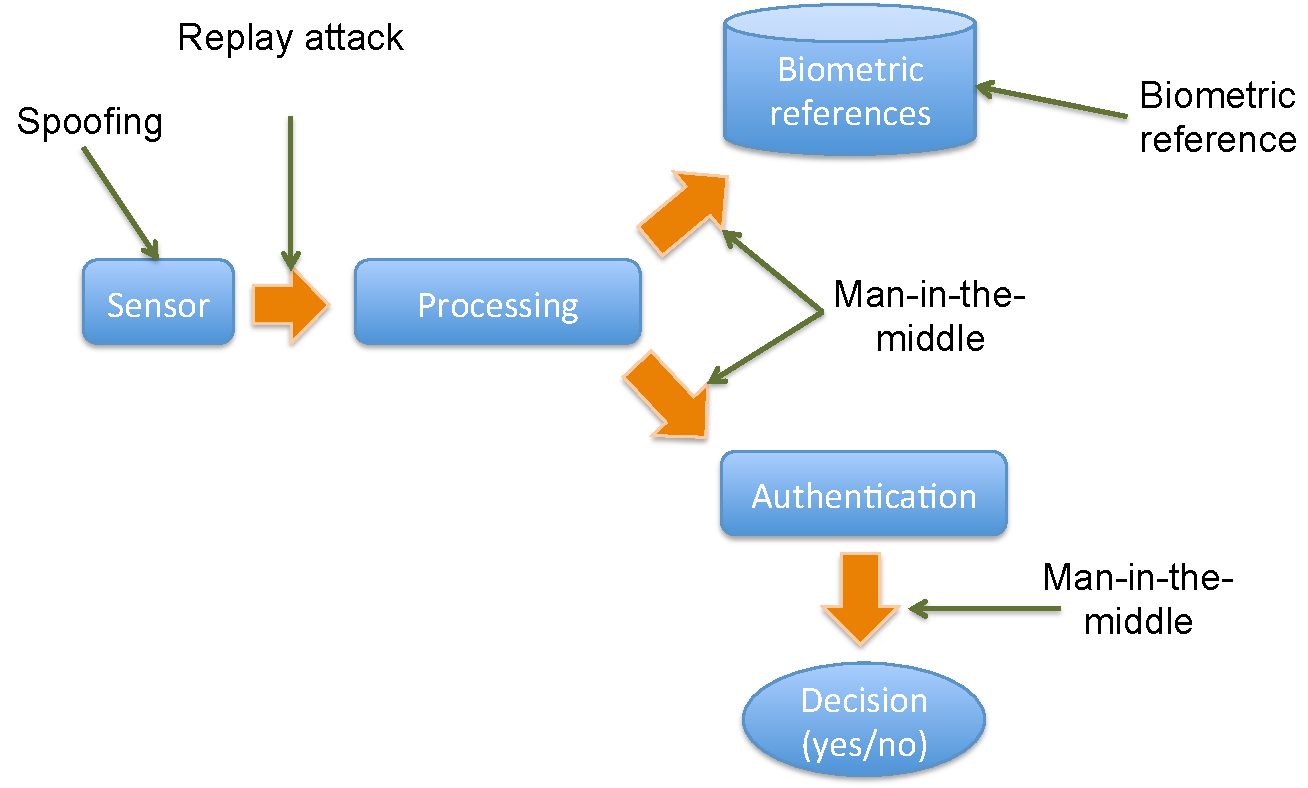
\includegraphics [width=14cm] {images/diagram_attacks.pdf}
\caption[]{ADAPATED FROM} \label{fig:diagram_attacks}
\end{center}
\end{figure}

Firstly the biometric trait is captured using some sensor. Secondly the captured biometric trait is processed in order to extract the biometric features. When it is in an enrolment procedure, these features will generate a biometric reference, and it will be stored in a database. In an authentication procedure, these features will be used in a comparison with the stored biometric reference. It is possible to observe in the same Figure that attacks can be done in any point of the architecture \cite{xiao2005security}. The next subsections will be discussed about each one of the possible point of attacks and how to mitigate it.


\label{sec:AttacksBiometric}

\subsection{Replay attack}

The replay attack is performed by injecting a biometric data previously sent, of the target identity, in order to have a non authorised access. This data can be obtained sniffing the biometric authentication software. To mitigate these kind of attacks, the biometric system should ensure that the provided data was not injected artificially \cite{xiao2005security}. The most  popular way of protect this kind of attack is to associate a timestamp to the data. As it is improbable to have the exactly the same biometric data in different times, this method is effective.

\subsection{Biometric reference attack}

The attack in the biometric reference is performed where the biometrics are stored. This kind of attack include actions such as the inclusion, removing, modifying and steal a biometric references. Among this actions, the possibility to steal a biometric reference is the most dangerous treat, since it is possible to work in a reverse engineering process to regenerate the biometric trait. 

Using a hill climbing technique to optimize to the position and the orientation of the minutia \cite{MartinezDiaz2006} and \cite{hill2001risk} shown that is possible to generate synthetic fingerprints compatible with fingerprints stored in a database. Fake fingers (with a real fingerprint) with gummy or silicon can be generated with this optimized minutia. It is possible also to inject these minutia in the \textbf{Processing} module (Figure \ref{fig:diagram_attacks}) in order to get a deceive the authentication system. 

To mitigate the risk of this kind of attack best practices in security recommends to encrypt the biometric references and to increase the policy to access these biometric references. 

\subsection{Man-in-the-middle}

In the man in the middle attack, the biometric data is intercepted to one point to another in any point of the architecture in Figure \ref{fig:diagram_attacks}.  As shown in the Figure, the attacker can, for example, manipulate the matching score; or inject a fake response or a fake biometric data (as shown in the replay attack) in order to get a forbidden access. 

\subsection{Ataque de Spoofing}

The spoofing attack in biometric system is a direct attack to the biometric sensor; a forged biometric is presented to the biometric sensor. The goal is to pretend to be someone else in order to get some forbidden privileges. This type of attack is described with more details in Chapter \ref{chap:Spoofing}.

Several technologies related to information security can be deployed in a biometric authentication system in order to mitigate the attacks aforementioned. We can highlight:
\begin{itemize}
        \item Encrypt the biometric data;
        \item Traffic the biometric data using a secure channel;
        \item Deploy all modules of the architecture in a device that cannot be broken;
        \item Using more than one authentication factor.
\end{itemize}
However, in a spoofing attack, the target is the biometric sensor, and in the chart presented in Figure \ref{fig:diagram_attacks}, is not possible to apply any of the security tools to prevent attacks, becoming the most fragile point of attack. This kind of attacks is the main point of this thesis.

\section{Final Remarks}
\label{sec:FinalRemarks}

This chapter described the main concepts and the main threats that can happen in biometric authentication systems. As aforementioned, the spoofing attacks are the most fragile point of threats in the architecture presented in the Figure \ref{fig:diagram_attacks}. Countermeasures need to be studied in order to mitigates these threats. This masters thesis will deal with that topic.




%Colocar o conteudo geral de spoofing neste cap.

\chapter{Spoofing Attacks}
\label{chap:Spoofing}

\section{Spoofing Attacks in Biometrics}
\label{sec:SpoofingAttacksBiometrics}

\section{Spoofing Attacks in Face Recognition}
\label{sec:SpoofingAttacksFaceRec}

\subsection{Presence of vitality (liveness)}
\subsection{Difference in motion patterns}
\subsection{Differences in image quality assessment}


\section{Face Spoofing Databases}
\label{sec:Databases}


\chapter{Developed Countermeasures}
\label{chap:Proposed_Countermeasures}

This chapter presents a countermeasure developed by the author in the scope of this masters dissertation. Micro-texture analysis has been effectively used in detecting photo attacks from single face images \cite{bai2010physics,maatta2011face,ChingovskaBIOSIG2012}. In this countermeasure the micro-texture analysis is extended to the spatiotemporal domain using the texture descriptor $LBP-TOP$ (Local Binary Patterns from Three Orthogonal Planes). The basic theory of Local Binary Patterns in spatiotemporal domain is introduced in Section \ref{sec_dynamic}. The architecture of the countermeasure is described in Section \ref{sec_proposed_counter}. In Section \ref{sec_experiments}, we report on the experimental setup and results. Finally, Section \ref{sec:Proposed_finalremarks} presents the Final Remarks of the chapter.

The content of this chapter was published in a satellite workshop of the Asian Conference in Computer Vision (ACCV - 2012) with the paper entitled "LBP-TOP based countermeasure against facial spoofing attacks" \cite{Pereira_LBP_2012}. Additionally this paper was extended and submitted to the journal "EURASIP Journal on Image Processing and Video Processing" organized by Springer with the paper entitled "Face liveness detection using dynamic texture" and is still under revision.

\section{LBP based dynamic texture description}
\label{sec_dynamic}

M\"{a}\"{a}tt\"{a} et al. \cite{maatta2011face} and Chingovska et al. \cite{ChingovskaBIOSIG2012} propose a $LBP$ based countermeasures to spoofing attacks based on the hypothesis that real faces  present different texture patterns in comparison with fake ones. However, the proposed techniques analyse each frame in isolation, not considering the behaviour over time. As aforementioned, in Chapter \ref{chap:Spoofing}, motion is a cue explored in some works and in combination with texture can generate a powerful countermeasure. For describing the face liveness for spoofing detection, we considered a spatiotemporal representation which combines facial appearance and dynamics. We adopted the $LBP$ based spatiotemporal representation because of its recent convincing performance in modeling moving faces and facial expression recognition and also for dynamic texture recognition \cite{inen2011computer}. 

The $LBP$ texture analysis operator, introduced by Ojala et al. \cite{ojala1996comparative,ojala2002multiresolution}, is defined as a gray-scale invariant  texture measure, derived from a general definition of texture in a local neighborhood. It is a powerful texture descriptor and among its properties in real-world applications are its discriminative power, computational simplicity and tolerance against monotonic gray-scale changes. The original $LBP$ operator forms labels for the image pixels by thresholding a 3$\times$3 neighborhood with the center value and considering the result as a binary number. The histogram of these $2^8=256$ different labels is then used as an image descriptor.

The original $LBP$ operator was defined to only deal with spatial information. However, more recently it has been extended to a spatiotemporal representation for dynamic texture analysis (DT). This has yielded to the so called Volume Local Binary Pattern operator ($VLBP$ \cite{zhao2007dynamic}. The idea behind $VLBP$ consists of looking at video sequence as a set of volumes in the ($X$,$Y$,$T$) space where $X$ and $Y$ denote the spatial coordinates and $T$ denotes the frame index (time). The neighborhood of each pixel is thus defined in a three dimensional space. Then, similarly to basic $LBP$ in spatial domain, volume textons can be defined and organized in histograms. Therefore, $VLBP$ combines motion and appearance into a dynamic texture description.

To make $VLBP$ computationally treatable and easy to extend, the co-occurrences of the $LBP$ on the three orthogonal planes ($LBP-TOP$) was also introduced \cite{zhao2007dynamic}. $LBP-TOP$ consists of the three orthogonal planes: $XY$, $XT$ and $YT$, and the concatenation of local binary pattern co-occurrence statistics in these three directions. The circular neighbourhoods are generalized to elliptical sampling to fit to the space-time statistics. The $LBP$ codes are extracted from the $XY$, $XT$ and $YT$ planes, which are denoted as $XY-LBP$, $XT-LBP$ and $YT-LBP$, for all pixels, and statistics of the three different planes are obtained, and concatenated into a single histogram. The procedure is shown in Figure \ref{fig:LBP-TOP_design}. In this representation, dynamic texture (DT) is encoded by the  $XY-LBP$, $XT-LBP$ and $YT-LBP$.

\begin{figure}[!htb]
\begin{center}
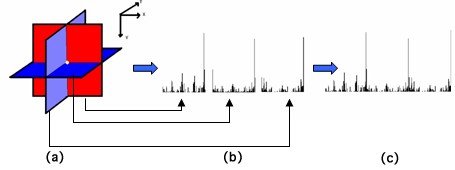
\includegraphics [width=0.75\linewidth] {images/proposed_countermeasure/LBP-TOP_design.png}
\caption[LBP-TOP scheme]{LBP-TOP scheme (a) Three planes intersecting one pixel (b) LBP histogram of each plane (c) Concatenating the histograms).} \label{fig:LBP-TOP_design}
\end{center}
\end{figure}
%(courtesy of \cite{zhao2007dynamic}

Using equal radii for the time and spatial axes is not a good choice for dynamic textures \cite{zhao2007dynamic} and therefore, in the $XT$ and $YT$ planes, different radii can be assigned to sample neighbouring points in space and time. More generally, the radii $R_{x}$, $R_{y}$  and $R_{t}$ respectively in axes X, Y and T , and the number of neighbouring points $P_{XY}$, $P_{XT}$ and $P_{YT}$ respectively in the $XY$, $XT$ and $YT$ planes can also be different. Furthermore, the type of $LBP$ operator on each plane can vary, for example the uniform pattern ($u2$) or rotation invariant uniform pattern ($riu2$) variants \cite{inen2011computer} can be deployed. The corresponding feature is denoted as $LBP-TOP_{P_{XY},P_{XT},P_{YT},R_{x},R_{y},R_{t}}^{operator}$.

Assuming we are given a $X\times Y \times T$ dynamic texture \\ $(x_c \in \left\{0,\cdots,X-1\right\},$ $y_c \in\left\{0,\cdots,Y-1\right\}, t_c\in\left\{0,\cdots,T-1\right\})$, i.e. a video sequence. An histogram of the DT can be defined as: 
\begin{equation}
%\begin{array}{ll}
H_{i,j}=\sum_{x,y,t}I\left\{f_{j}(x,y,t)=i\right\},\enspace i=0,\cdots,n_j-1;j=0,1,2 \enspace.
%\end{array}
\end{equation}
where $n_j$ is the number of different labels produced by the LBP operator in the $j_{th}$ plane ($j=0: XY,~1: XT~and~2: YT$), $f_i(x,y,t)$ expresses the LBP code of central pixel $(x,y,t)$ in the $j_{th}$ plane and $I$ is defined as follows:

\begin{equation}
I(A) = \left\{ 
  \begin{array}{l l}
    1 &  \textrm{if $A$ is true}\\
    0 &  \textrm{if $A$ is false.}\\
  \end{array} \right.
\end{equation}

%in which $n_j$  is the number of different labels produced by the LBP operator in the $j$th plane ($j=0: XY,~1: XT~and~2: YT$) and $f_i(x,y,t)$ expresses the LBP code of central pixel $(x,y,t)$ in the $j$th plane.

Similarly to the original LBP, the histograms are normalized to get a coherent description for comparing the DTs:
\begin{equation}
N_{i,j}=\frac{H_{i,j}}{\sum_{k=0}^{n_j-1}H_{k,j}} \enspace .
\end{equation}

In addition to the computational simplification, compared with $VLBP$, $LBP-TOP$ has the advantage to generate independent histograms for each of intersecting planes, in space and time, which can be treated in combination or individually. Because of the aforementioned complexity issues on the implementation of a $VLBP$ based processor, the developed spatiotemporal face liveness description uses $LBP-TOP$ to encode both facial appearance and dynamics. 

The key idea of this countermeasure is to learn and detect the structure and the dynamics of the facial micro-textures that characterize real faces but not fake ones. Due to its tolerance against monotonic gray-scale changes, $LBP$ based representation is a large used descriptor for measuring the facial texture quality and determining whether degradations due to recapturing process, e.g. the used spoofing medium, are observed. Instead of just applying static texture analysis, we exploit also several dynamic visual cues that are based on either the motion patterns of a genuine human face or the used display medium.

\begin{figure}[!htb]
\begin{center}
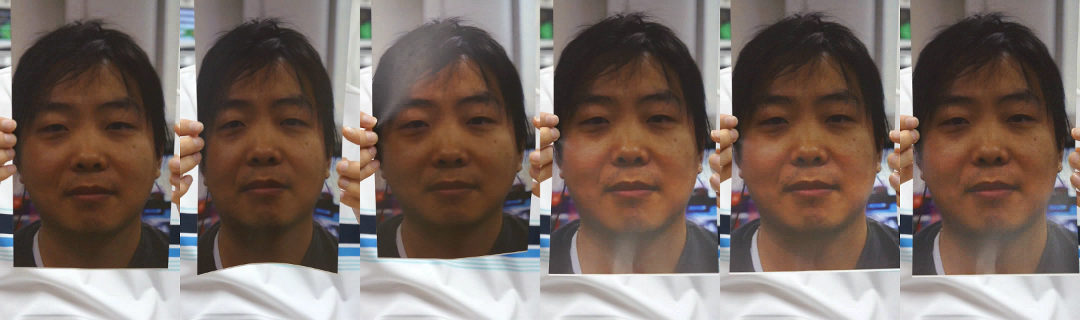
\includegraphics [width=0.85\linewidth] {images/proposed_countermeasure/flicker.png}
\caption[Sequence of a warped photo attack extracted from the CASIA FASD]{Sequence of a warped photo attack extracted from the CASIA FASD \cite{zhangface} describing the characteristic reflections (flickering) of planar spoofing medium and the distorted motion patterns.} \label{fig:flickering}
\end{center}
\end{figure}
%\cite{zhangface}

Unlike photographs and display devices, real faces are indeed non-rigid objects with contractions of facial muscles which result in temporally deformed facial features such as eye lids and lips. Therefore, it can be assumed that the specific facial motion patterns (including eye blinking, mouth movements and facial expression changes) should be detected when a live human being is observed in front of the camera. The movement of the display medium may cause several distinctive motion patterns that do not describe genuine faces. As shown in Figure \ref{fig:flickering} (between the second and the third picture), the use of (planar) spoofing medium might cause sudden characteristic reflections when a photograph is warped or because of a glossy surface of the display medium. As it can be seen, warped photo attacks may cause also distorted facial motion patterns. It is likely that hand-held attacks introduce synchronized shaking of the face and spoofing medium which can be observed as excessive relative motion in the view and facial region if the distance between the display medium and the camera is relatively short. Our countermeasure tries to exploit the aforementioned visual cues for face spoofing detection by exploring the dynamic texture content of the facial region. We adopted the $LBP$ based spoofing detection in spatiotemporal domain because $LBP-TOP$ features have been successfully applied in describing dynamic events, e.g. facial expressions \cite{zhao2007dynamic}.

%%%%%%%%%%%%%%%%%%%%%%
%%%%%%%%%%%%%%%%%%%%%%
% The proposed counter measure
%%%%%%%%%%%%%%%%%%%%%%
%%%%%%%%%%%%%%%%%%%%%%

\begin{figure}[!htb]
\begin{center}
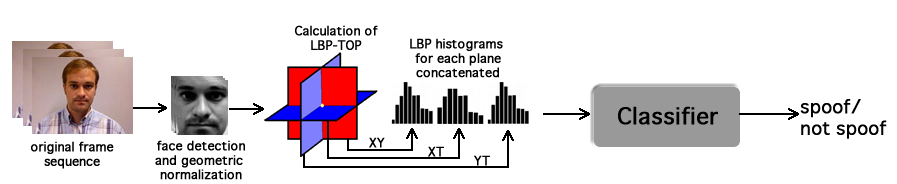
\includegraphics [width=16cm] {images/proposed_countermeasure/countermeasure_2.png}
\caption[Block diagram of the proposed countermeasure based on LBP-TOP]{Block diagram of the proposed countermeasure based on LBP-TOP} \label{fig_countermeasure}
\end{center}
\end{figure}

\section{Architecture of the countermeasure}
\label{sec_proposed_counter}

Figure \ref{fig_countermeasure} shows a block diagram of the proposed countermeasure. First, each frame of the original frame sequence was gray-scaled and passed through a face detector using Modified Census Transform ($MCT$) features \cite{froba2004face}. Only detected faces with more than 50 pixels of width and height were considered. The detected faces were geometric normalized to 64$\times$64 pixels. The bounding box returned by the automatic face detector, introduce some noises in the $LBP-TOP$ description. The bounding box, in general, is slightly dislocated in successive frames, even without a translational movement. The $LBP-TOP$ descriptor can register movement with this noise. In order to reduce this kind of noise, the same face bounding box was used for each set of frames used in the $LBP-TOP$ calculation. As can be seen in the Figure \ref{fig_faceDetection}, the middle frame was chosen. Unfortunately, the face detector is not error free and in case of error in the middle frame face detection, the nearest detection was chosen. If there is not detected face, in the observed time window, the observation was discarded. After the face detection step, the $LBP$ operators were applied for each plane ($XY$, $XT$ and $YT$) and the histograms were computed and then concatenated. After the feature extraction step, binary classification can be used to discriminate spoofing attacks from real access attempts.

\begin{figure}[!htb]
\begin{center}
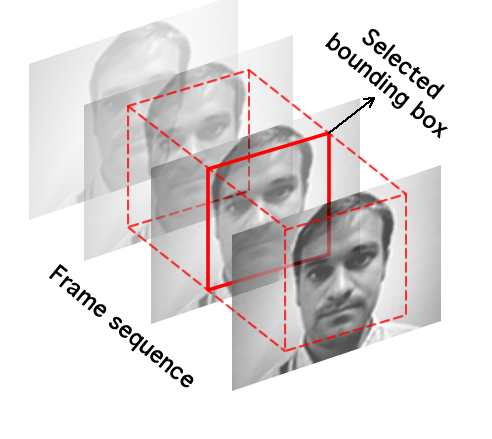
\includegraphics [width=6cm] {images/proposed_countermeasure/faceDetection_2.png}
\caption[Face detection strategy for $R_t = 1$]{Face detection strategy for $R_t = 1$} \label{fig_faceDetection}
\end{center}
\end{figure}

Face liveness is rather difficult to be determined based on the motion between couple of successive frames. The used volume can be expanded along the temporal dimension by increasing $R_t$, as aforementioned in section \ref{sec_dynamic}. This way to deal with dynamic texture is called single resolution approach, since only one histogram per $LBP-TOP$ plane is accumulated. However, this leads to rather sparse sampling on the temporal planes $XT$ and $YT$, thus we might loose valuable details. In order to explore the dynamic texture information more carefully, we proposed the multiresolution approach.

The multiresolution approach can be performed by concatenating the histograms in the time domain ($XT$ and $YT$) for different values of $R_t$. The notation chosen to represent these settings is using brackets for the multiresolution data. For example, $R_t=[1-3]$ means that the LBP-TOP operator will be calculated for $R_t=1$, $R_t=2$ and $R_t=3$ and all resultant histograms will be concatenated. With the multiresolution approach, dense sampling on the temporal planes $XT$ and $YT$ is achieved.

%The proposed countermeasure was implemented using the free signal processing and machine learning toolbox Bob \cite{AnjosIdiapRR252012} and the source code of the algorithm is available as an add-on package to this framework$^3$. After installation, it is possible to reproduce all results reported in this article.

%%%%%%%%%%%%%%%%%%%%%%
%%%%%%%%%%%%%%%%%%%%%%
% Experiments
%%%%%%%%%%%%%%%%%%%%%%
%%%%%%%%%%%%%%%%%%%%%%
\section{Experiments}
\label{sec_experiments}

This section provides an in-depth analysis on the proposed $LBP-TOP$ based face liveness description using the Replay Attack Database \cite{ChingovskaBIOSIG2012} and the CASIA FASD \cite{zhangface}. The $LBP-TOP$ representation is computed over relatively short temporal windows and the results are reported using the overall classification accuracy for the individual volumes. Altogether four experiments were carried out evaluating the effectiveness of:

\begin{enumerate}
        \item Each $LBP-TOP$ plane individually and in combination;
        \item Different classifiers;
        \item Different LBP operators;
        \item The multiresolution approach.
\end{enumerate}

In order to study the effect of the different variables, each parameter was tuned solely (fixing other elements) using the development set of each face spoofing database. It should be noted that unlike the Replay Attack Database, the CASIA FASD lacks a specific development set. Therefore, the first four experiments were performed in this database using cross-validation by randomly dividing the training data into five folds. Hence, the results presented for CASIA FASD are actually the average $HTER$ on the test set over five iterations of the algorithm with different folds playing the role of a development set.

Finally, we also studied the accumulation of facial appearance and dynamics information over longer time windows and perform an evaluation at system level. The access attempt based results presented in Section \ref{sec_attempt} were obtained using the official protocol of each database.

Inspired by \cite{ChingovskaBIOSIG2012}, the $LBP-TOP$ operator chosen to start the evaluation was $LBP-TOP_{8,8,8,1,1,R_{t}}^{u2}$. 

%--------------------------------------------------------------------------------------------------------
\subsection{Effectiveness of each $LBP-TOP$ plane individually and in combination}
\label{sec_lbptop_planes}

In this experiment, we analysed the effectiveness of each individual plane and their combinations when the multiresolution area is increased. Figure \ref{fig:planes_evaluation_LDA} shows the $HTER$ evolution, on the test set, considering individual and combined histograms of $LBP-TOP$ planes for each database. We used, as binary classifier, a linear projection derived from LDA (Linear Discriminant Analysis) as in \cite{ChingovskaBIOSIG2012}.

\begin{figure}[!htb]
\begin{center}
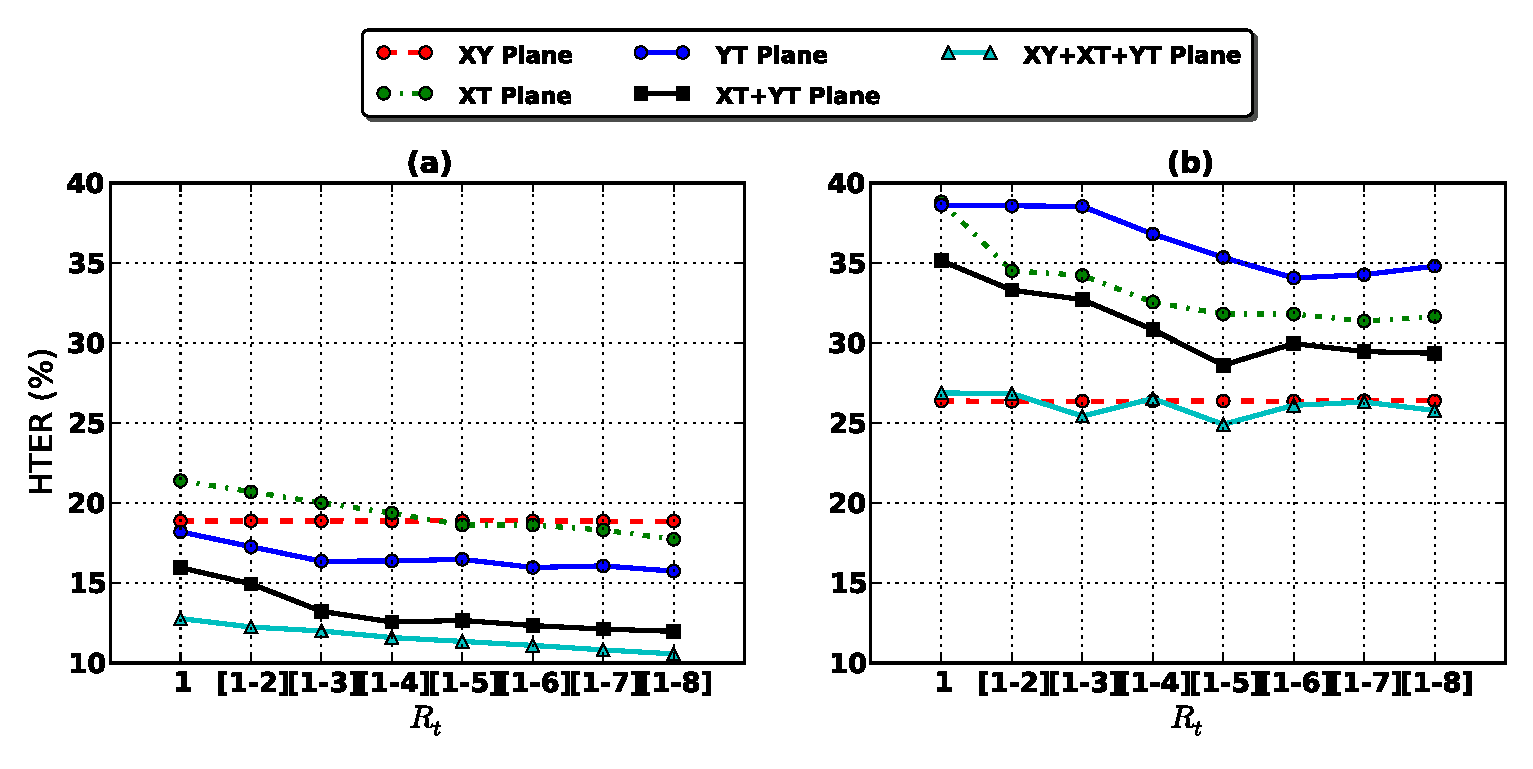
\includegraphics [width=\textwidth] {images/proposed_countermeasure/planes_evaluation_LDA.pdf}
\caption[HTER(\%) evaluation in each plane when the multiresolution area ($R_t$) is increased]{HTER(\%) evaluation in each plane when the multiresolution area ($R_t$) is increased with LBP-TOP$_{8,8,8,1,1,R_t}^{u2}$ and LDA classifier - test-set \textbf{(a)} Replay Attack Database \textbf{(b)} CASIA FASD.} \label{fig:planes_evaluation_LDA}
\end{center}
\end{figure}

The results indicate differences in the performance between the two databases. The temporal components ($XT$ and $YT$) are a decisive cue for the Replay Attack Database and the combination of all three planes ($XY$, $XT$ and $YT$) gives the best performance. Conversely, for the CASIA FASD, the addition of temporal planes improves the performance only slightly compared to the spatial $LBP$ representation (considering only the $XY$ plane). These observations can be explained by taking a closer look at the differences in the databases and their spoofing attack scenarios. 2D fake face attacks can be categorized into two groups, close-up and scenic attacks, based on how the fake face is represented with the spoofing medium.

A close-up spoof describes only the facial area which is presented to the sensor. The main weakness with the tightly cropped fake faces is that the boundaries of the spoofing medium, e.g. a video screen frame, photograph edges, or the attacker's hands are usually visible during the attack, thus can be detected in the scene \cite{JukkaLBP2012}. However, these visual cues can be hidden by incorporating background scene in the face spoof and placing the resulting scenic fake face very near to the sensor as performed on the Replay Attack Database. In such cases, the description of facial appearance leads to rather good performance because the proximity between the spoofing medium and the camera causes the recaptured face image to be out-of-focus also revealing other facial texture quality issues, like degradation due to the used spoofing medium. Furthermore, the attacks in Replay Attack Database are performed using two types of support conditions, fixed and hand-held. Naturally, the $LBP-TOP$ based face representation can easily detect fixed photo and print attacks since there is no variation in the facial texture over time. On the other hand, the hand-held attacks introduce synchronized shaking of the face and spoofing medium. This can be observed as excessive relative motion in the view, again, due to the proximity between the display medium and the sensor. Since the distinctive global motion patterns are clearly visible also on the facial region, they can be captured even by computing the LBP-TOP description over relatively short temporal windows, i.e. low values of $R_t$.

In contrast, the CASIA FASD consists of close-up face spoofs. The distance between the camera and the display medium is much farther compared to the attacks on Replay Attack Database. The display medium does not usually move much in the attack scenarios. Therefore, the overall translational movement of a fake face is much closer to the motion of a genuine head. Due to the lack of distinctive shaking of the display medium, the CASIA FASD can be considered to be more challenging from the dynamic texture point of view. Because the motion cues are harder to explore in some attack scenarios using small values of $R_t$, we investigated in Section \ref{sec_attempt} whether the use of longer time windows helps to reveal the disparities between a genuine face and a fake one.


%--------------------------------------------------------------------------------------------------------
\subsection{Effectiveness of different classifiers}
\label{sec_different_classifiers}

In this experiment, we analysed the effectiveness of different classifiers when the multiresolution area is increased. Fig. \ref{fig:evaluation_classifiers} shows the HTER evolution, on the test set, under three different classifications schemes. The first one uses $\chi^2$ distance, since the feature vectors are histograms. The same strategy reported in \cite{ChingovskaBIOSIG2012} was carried out. A reference histogram only with real accesses was created averaging the histograms in the training set. The last two selected classification schemes analysed were: Linear Discriminant Analysis (LDA) and Support Vector Machines (SVM) with a radial basis function kernel (RBF).

\begin{figure}[!btb]
\begin{center}
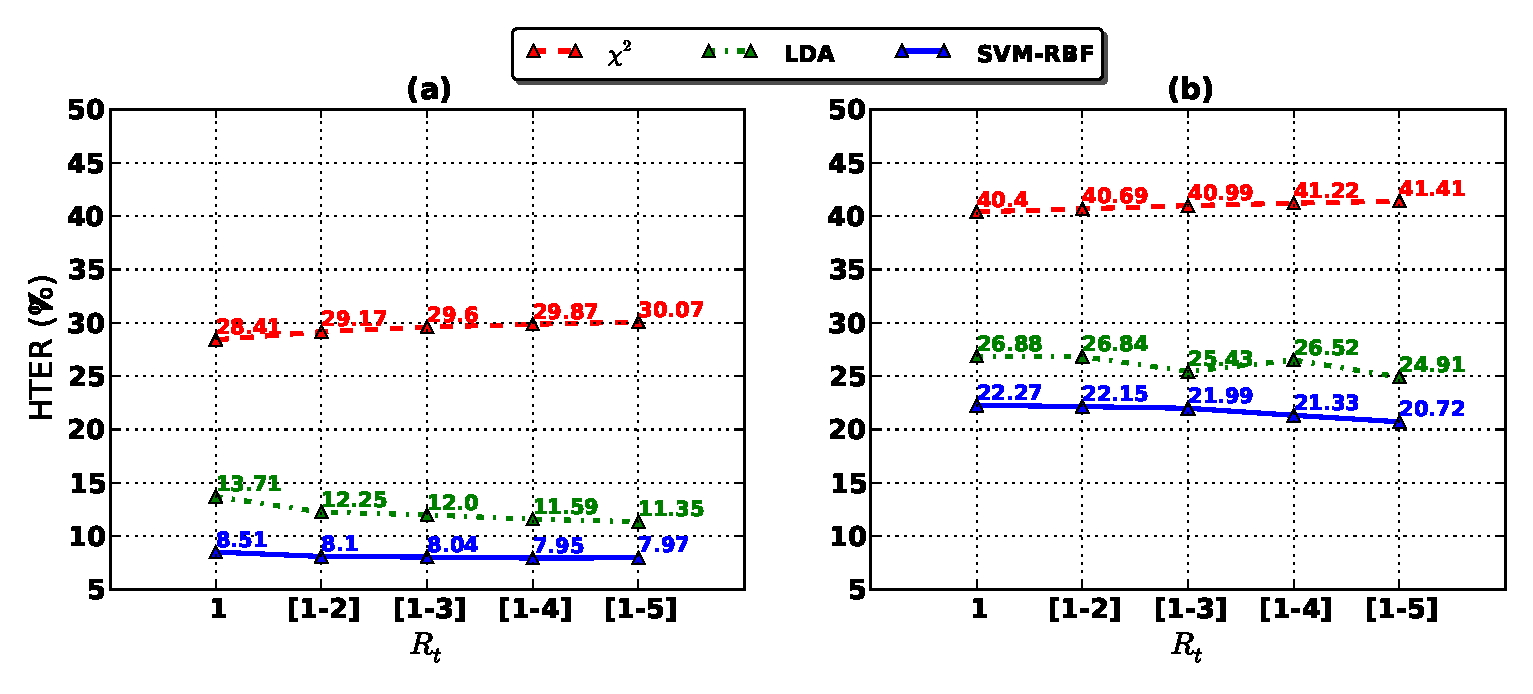
\includegraphics [width=\textwidth] {images/proposed_countermeasure/evaluation_classifiers.pdf}
\caption[HTER(\%) evaluation with LBP-TOP$_{8,8,8,1,1,R_t}^{u2}$ using different classifiers]{HTER(\%) evaluation with LBP-TOP$_{8,8,8,1,1,R_t}^{u2}$ using different classifiers \textbf{(a)} Replay Attack Database \textbf{(b)} CASIA FASD.} \label{fig:evaluation_classifiers}
\end{center}
\end{figure}


The SVM classifier with an RBF kernel provided the best performance on the Replay Attack Database and the CASIA FASD (7.97\% and 20.72\% in terms of HTER, respectively). However, it is important to remark that the same LBP-TOP configuration with an LDA classifier resulted in comparable performance (11.35\% and 24.91\% in terms of HTER). This is not a huge gap and the classification scheme is far simpler. As similar findings have been reported \cite{ChingovskaBIOSIG2012,Komulainen_ICB_2013}, the use of simple and computationally efficient classifiers should be indeed considered when constructing real-world anti-spoofing solutions.


%--------------------------------------------------------------------------------------------------------
\subsection{Effectiveness of different LBP operators}
\label{sec_different_lbp_operators}


The size of the histogram in a multiresolution analysis, in time domain, increases linearly with $R_t$. The choice of an appropriate LBP representation in the planes is an important issue since it impacts the size of the histograms. Using uniform patterns or rotation invariant extensions, in one or multiple planes, may bring a significant reduction in computational complexity. In this experiment, the effectiveness of different LBP operators in the three LBP-TOP planes ($XY$, $XT$ and $YT$) was analysed. Fig. \ref{fig:evaluation_LBP-operator} shows the performance, in HTER terms, configuring each plane as basic LBP (with 256 bins for $P=8$), LBP$^{u2}$ (uniform patterns) and LBP$^{riu2}$ (rotation invariant uniform patterns) when the multiresolution area ($R_t$) is increased in both databases. Results must be interpreted with the support of Fig. \ref{fig:dimIncrease}, which shows the number of bins on the histograms used for classifications in each configuration.


\begin{figure}[!btb]
\begin{center}
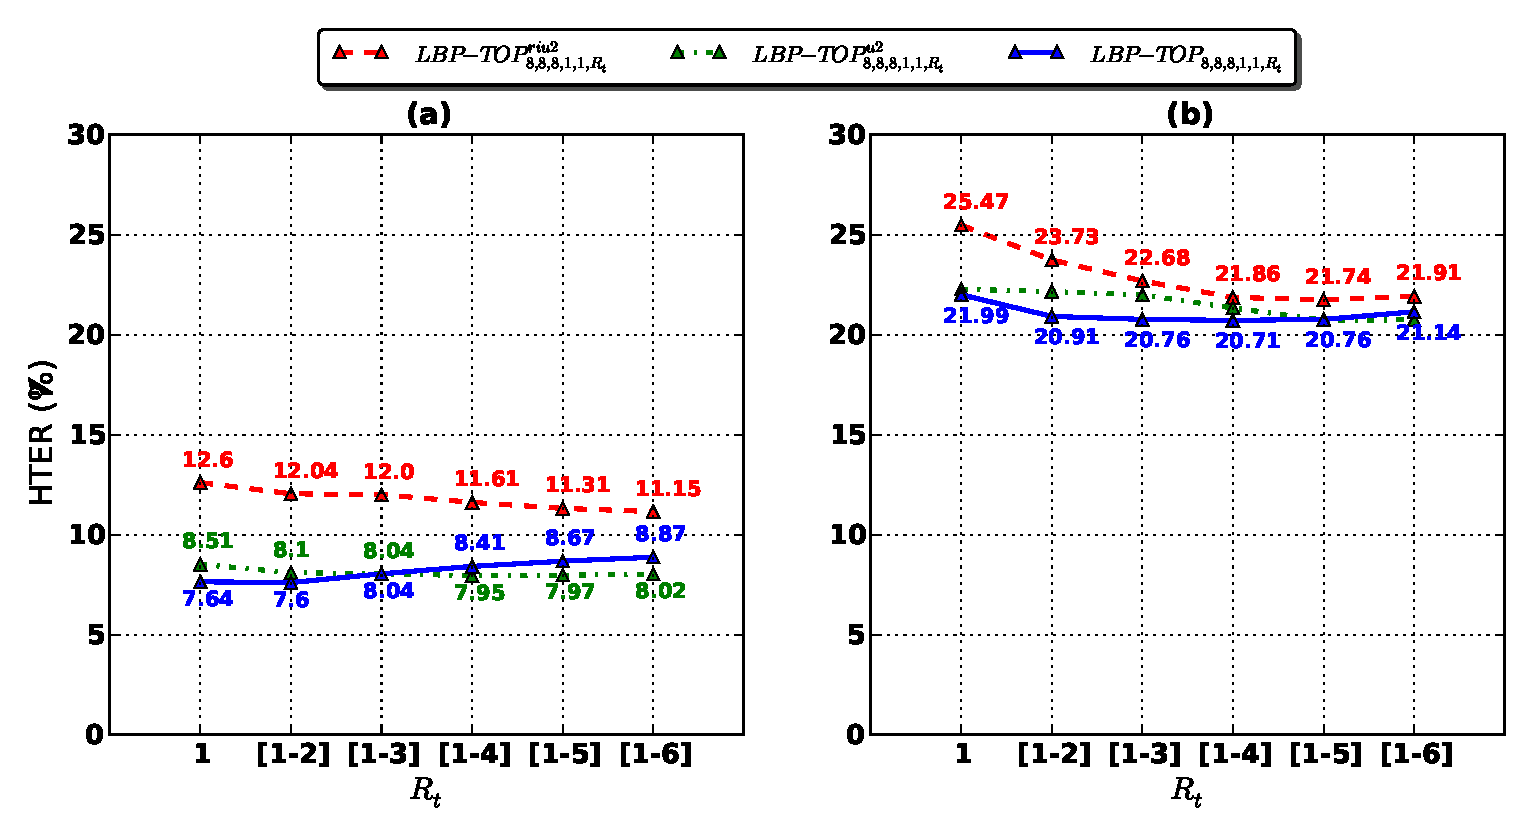
\includegraphics [width=\textwidth] {images/proposed_countermeasure/evaluation_LBP-operator.pdf}
\caption[HTER(\%) evaluation with LBP-TOP$_{8,8,8,1,1,R_t}$ using different LBP operators]{HTER(\%) evaluation with LBP-TOP$_{8,8,8,1,1,R_t}$ using different LBP operators in the planes with SVM classifier \textbf{(a)} Replay Attack Database \textbf{(b)} CASIA FASD.}
\label{fig:evaluation_LBP-operator}
\end{center}
\end{figure}

\begin{figure}[!btb]
\begin{center}
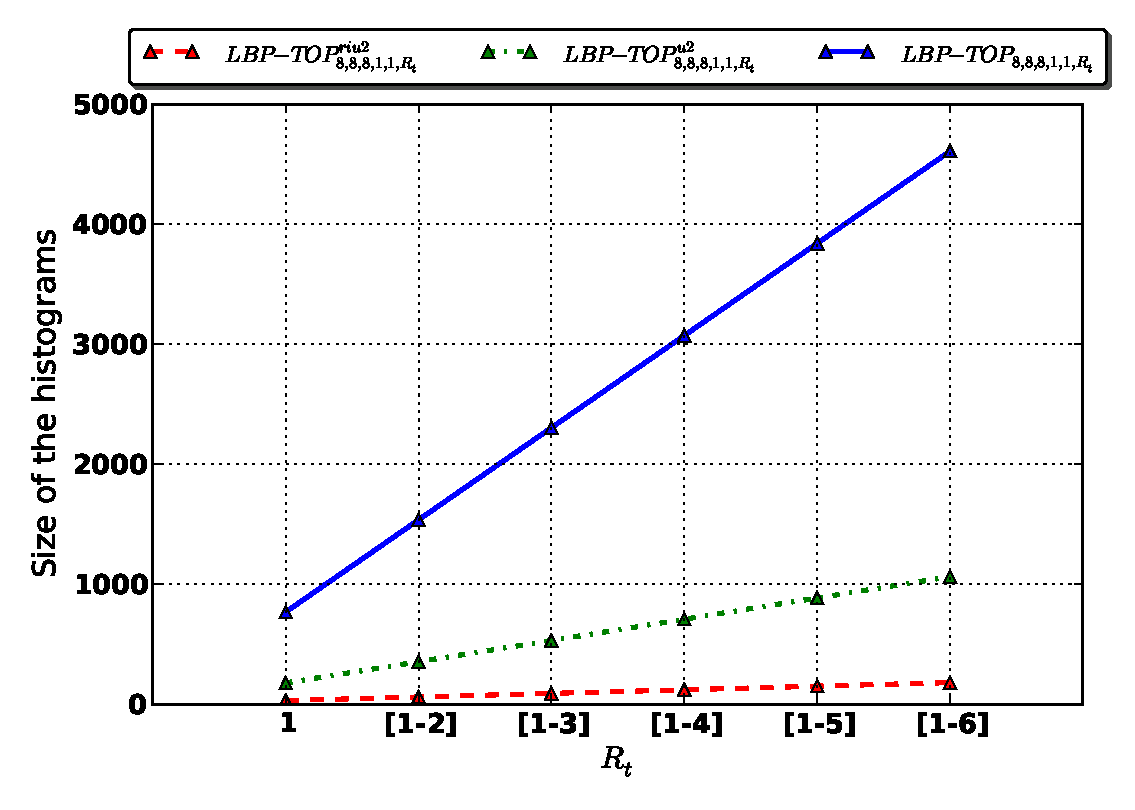
\includegraphics [width=10cm] {images/proposed_countermeasure/dimIncrease.pdf}
\caption{Evaluation of the histogram size when ($R_t$) is increased.} 
\label{fig:dimIncrease}
\end{center}
\end{figure}

When the multiresolution area is increased, the HTER saturates for LBP$^{riu2}$ and LBP$^{u2}$ on both datasets. For the basic LBP operator a minimum can be observed in 7.60\% and 20.71\% on the Replay Attack Database and CASIA FASD respectively. On both databases, basic LBP and LBP$^{u2}$ presented similar performance. Even though the use of regular LBP leads to the best results, the LBP$^{u2}$ operator seems to provide a reasonable trade-off between computational complexity (see Fig. \ref{fig:dimIncrease}) and performance. Hence, we will still proceed with LBP$^{u2}$.

%--------------------------------------------------------------------------------------------------------
\subsection{Effectiveness of the multiresolution approach}
\label{sec_multiresolution}

In this experiment we analysed the effectiveness of the multiresolution approach in comparison to the single resolution approach. The single resolution approach consists of using only fixed values for $R_t$, without concatenating histograms for each $R_t$. With this approach the size of the histograms will be constant for different values of $R_t$, which decreases the computational complexity compared to the multiresolution approach. Fig. \ref{fig:multiVSsingle} shows the HTER evolution for different values of $R_t$ in both databases comparing the both approaches.

\begin{figure}[!htb]
\begin{center}
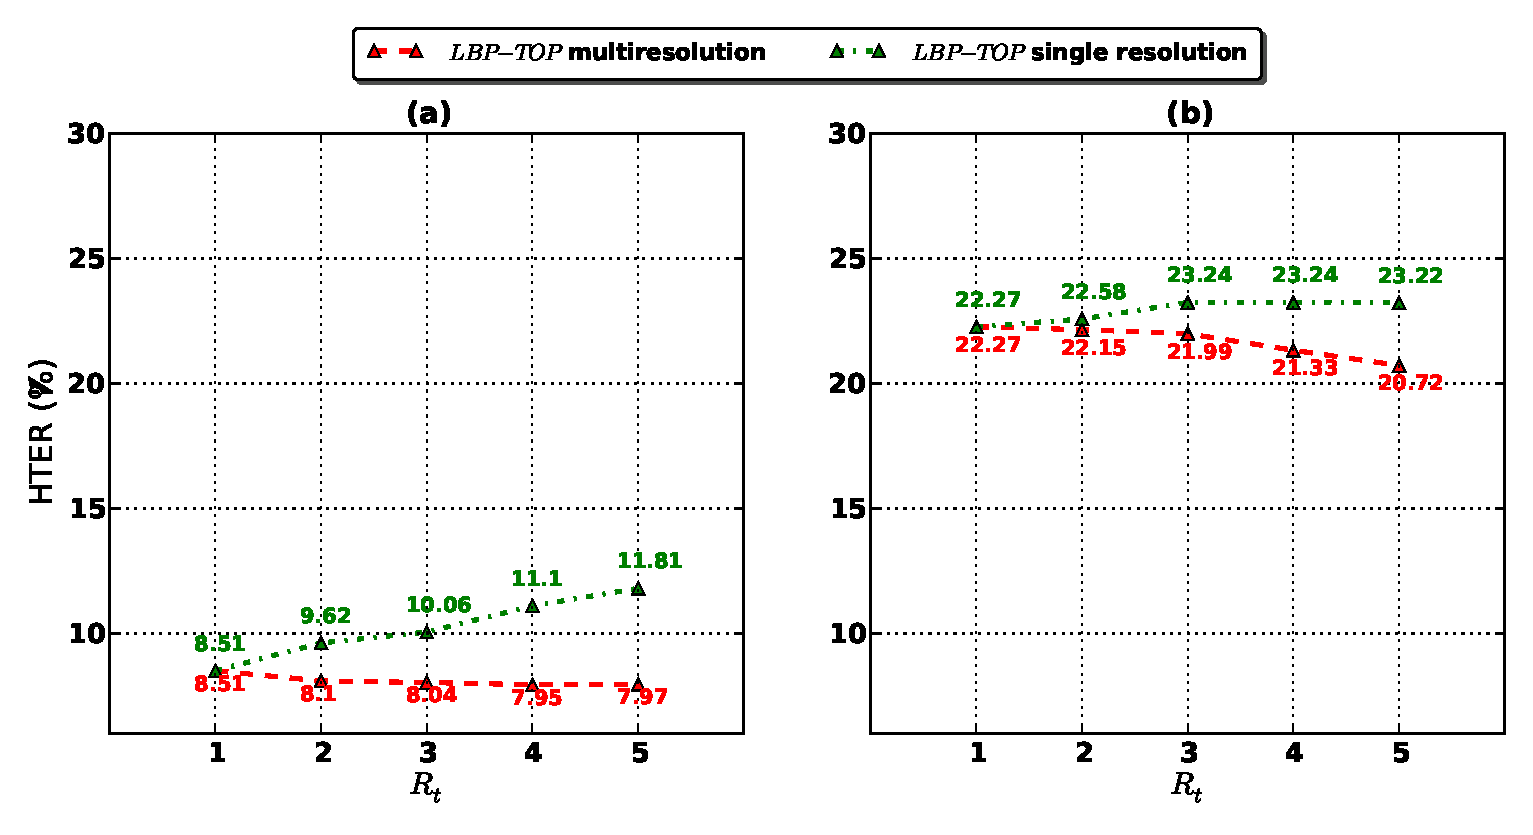
\includegraphics [width=\textwidth] {images/proposed_countermeasure/multiVSsingle.pdf}
\caption[HTER(\%) evaluation using LBP-TOP$_{8,8,8,1,1,R_t}^{u2}$ with the single resolution and the multiresolution approach]{HTER(\%) evaluation using LBP-TOP$_{8,8,8,1,1,R_t}^{u2}$ with the single resolution and the multiresolution approach using SVM classifier \textbf{(a)} Replay Attack Database \textbf{(b)} CASIA FASD.} \label{fig:multiVSsingle}
\end{center}
\end{figure}


On both datasets, the HTER of single resolution approach increases with $R_t$ whereas the multiresolution approach helps to keep the HTER low when the multiresolution area is increased. This suggests that the increase of $R_t$ causes more sparse sampling in the single resolution approach when valuable motion information is lost. In contrary, the more dense sampling of the multiresolution approach is able to provide a more detailed description of the motion patterns, thus improving the discriminative power.

%--------------------------------------------------------------------------------------------------------

\subsection{Access attempt based analysis}
\label{sec_attempt}

In the previous experiments, the importance of the temporal dimension was studied using the single resolution and the multiresolution approaches. As presented in Section\ref{sec_lbptop_planes}, the multiresolution approach is able to capture the nature of fixed photo attacks and the excessive motion of display medium, especially on the Replay Attack Database. However, in some attack scenarios, the motion patterns were harder to explore using small values of $R_t$. We now study how the temporal window size affects the performance when the facial appearance and dynamics information are accumulated over time. The face description of the single resolution and multiresolution methods can be accumulated over longer time periods either by averaging the features within a time window or by classifying each subvolume and then averaging the scores within the current window. In this manner, we are able to provide dense temporal sampling over longer temporal windows without excessively increasing the size of the feature histogram.

In order to follow the method used in previous experiments, we begin evaluating the two averaging strategies with the LBP-TOP$_{8,8,8,1,1,1}^{u2}$ operator and a SVM classifier with RBF kernel. In order to determine the video based system performance, we applied both average of features and scores on the first valid time window of N frames from the beginning of each video sequence. It should be noted that the following access attempt based analysis is based on the official protocol of each database. Thus, the results on Replay Attack Database are reported in terms of HTER whereas the performance on CASIA FASD is described using EER.

The access attempt based performance of both averaging strategies on the two databases is presented in Fig. \ref{fig:blocks_in_videos}. The results indicate that when the amount of temporal information increases, the better we are able to discriminate real faces from fake ones. This is the case especially on the CASIA FASD in which the distinctive motion clues, such as the excessive shaking of the display medium, cannot be exploited. However, when longer video sequences are explored, we are more likely to observe other specific dynamic events, such as different facial motion patterns (including eye blinking, lip movements and facial expression changes) or sudden characteristic reflections of planar spoofing media which can be used for differentiating real faces from fake ones. It is also interesting to notice that by averaging features, more stable and robust spoofing detection performance is achieved on both databases. The averaging scores of individual sub-volumes seems to suffer from outliers, thus more sophisticated temporal processing of scores might lead to more stable behavior.


\begin{figure}[h]
\begin{center}
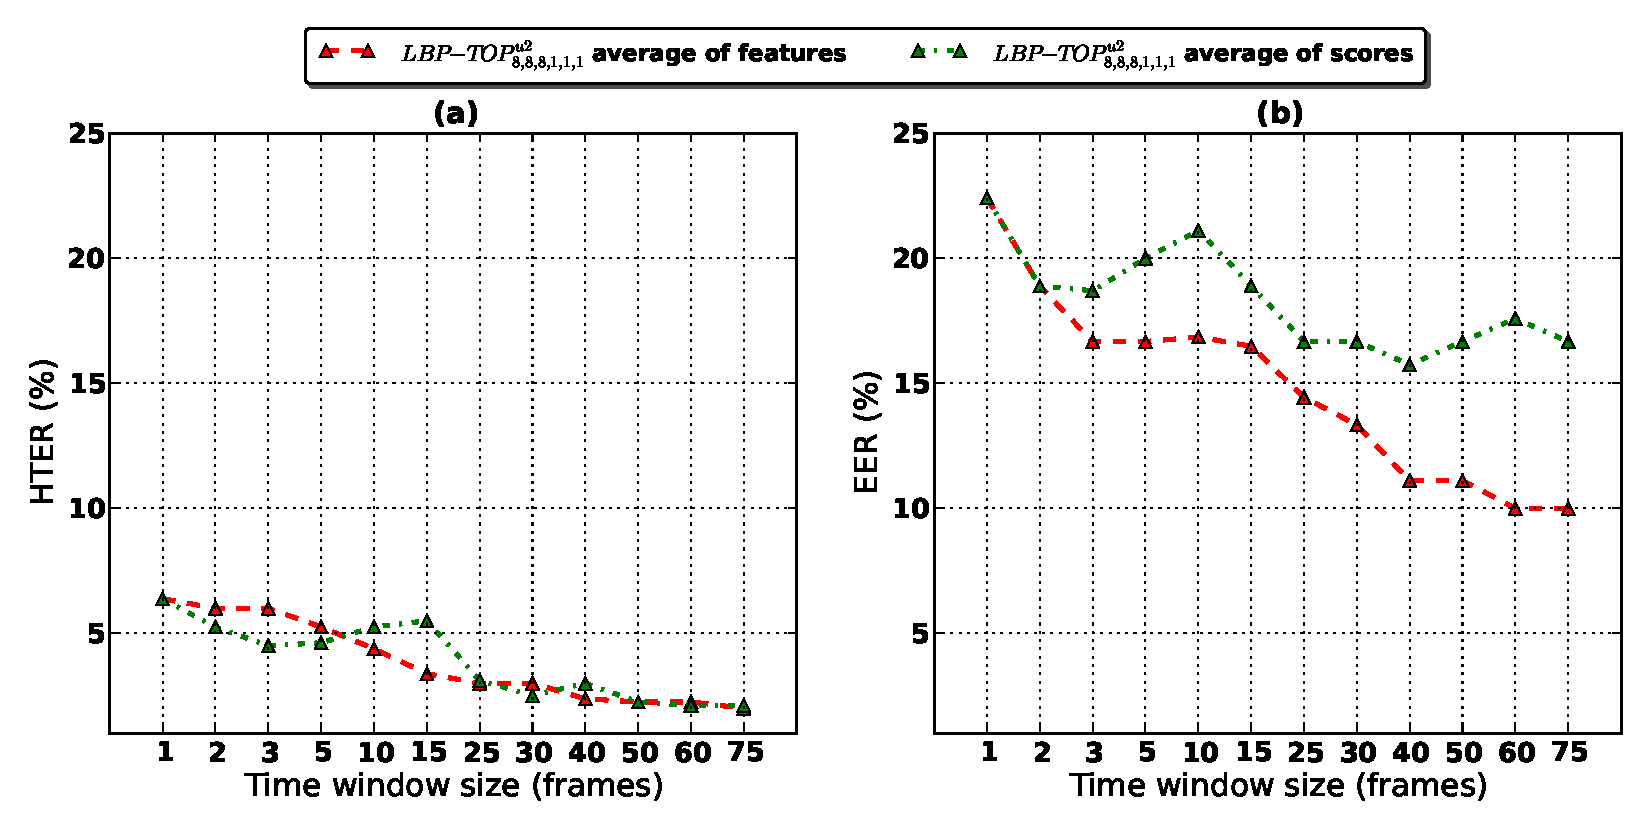
\includegraphics [width=\textwidth] {images/proposed_countermeasure/video_based_results.pdf}
\caption[Access attempt based evaluation of different time window sizes]{Access attempt based evaluation of different time window sizes using mean of features and mean of scores with LBP-TOP$_{8,8,8,1,1,1}^{u2}$(a) Replay Attack Database (HTER \%) (b) CASIA FASD (EER \%).} \label{fig:blocks_in_videos}
\end{center}
\end{figure}

According to the official test protocol of CASIA FASD, also the DET curves and the EERs for the seven scenarios (Section \ref{sec_casia}) should be reported. Based on the previous analysis we chose to use the average of features within a time window of 75 frames which corresponds to three seconds of video time. As it can be seen in Fig \ref{fig:DET_overall} and Table \ref{tab:casia_eer}, the use of only facial appearance (LBP) leads to better results compared to the baseline method (CASIA FASD baseline). More importantly, when the temporal planes XT and YT are also considered for spatiotemporal face description (LBP-TOP), a significant performance enhancement is obtained (from 16\% to 10\% in terms of EER), thus confirming the benefits of encoding and exploiting not only the facial appearance but also the facial dynamics information.


\begin{figure}[h]
\begin{center}
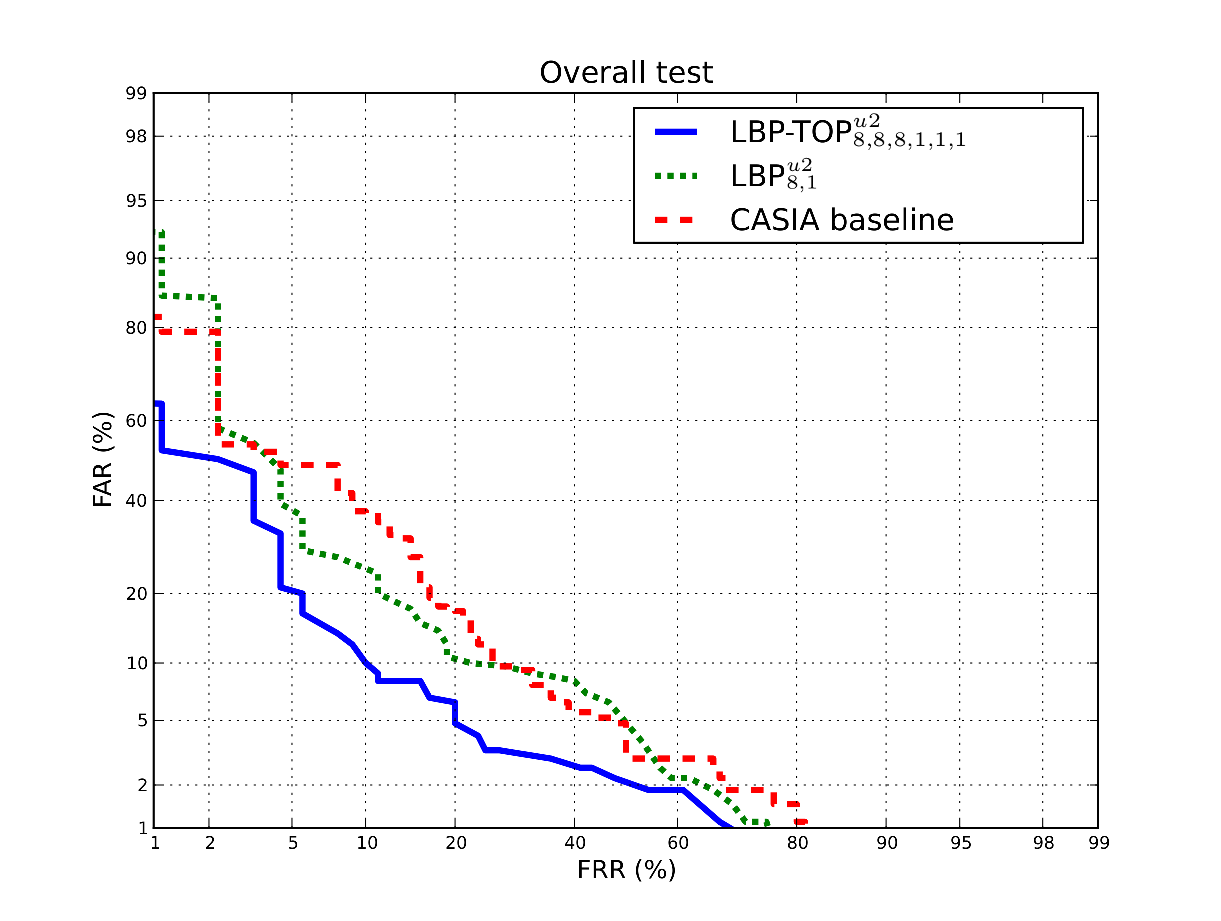
\includegraphics [width=0.6\linewidth] {images/proposed_countermeasure/casia_scenarios_XYT_XY_baseline.pdf}
\caption[Overall performance of LBP-TOP$_{8,8,8,1,1,1}^{u2}$ using average of features compared to the DoG baseline method]{Overall performance of LBP-TOP$_{8,8,8,1,1,1}^{u2}$ using average of features compared to the DoG baseline method and LBP$_{8,1}^{u2}$ on the CASIA FASD.} 
\label{fig:DET_overall}
\end{center}
\end{figure}

\begin{table}
\caption{EER (in \%) comparison between the DoG baseline method, LBP$_{8,1}^{u2}$ and LBP-TOP$_{8,8,8,1,1,1}^{u2}$ using average of features on the CASIA FASD.}
\begin{center}
\begin{tabular}{|c|c|c|c|c|c|c||c|}
\hline 
Scenario & Low & Normal & High & Warped & Cut & Video & Overall\\
\hline 
DoG baseline \cite{zhangface} & {\centering 13} & {\centering 13} & {\centering 26} & {\centering 16} & {\bf \centering 6} & {\centering 24} & {\centering 17}\\
\hline 
LBP$_{8,1}^{u2}$ & {\centering 11} & {\centering 17} & {\bf \centering 13} & {\centering 13} & {\centering 16} & {\centering 16} & {\centering 16}\\
\hline 
LBP-TOP$_{8,8,8,1,1,1}^{u2}$ & {\bf \centering 10} & {\bf \centering 12} & {\bf \centering 13} & {\bf \centering 6} & {\centering 12} & {\bf \centering 10} & {\bf \centering 10}\\
\hline 
\end{tabular}
\end{center}
\label{tab:casia_eer}
\end{table}

More detailed results for each scenario are presented in Fig. \ref{fig:DET_protocols} and in Table \ref{tab:casia_eer}. The results indicate that the proposed LBP-TOP based face description yields best results in all configurations except under cut-photo attacks. As described in \cite{zhangface}, the DoG filtering baseline method is able to capture the less variational nature of the cut eye regions well. However, the difference in the motion patterns seems to be too small for our LBP-TOP based approach as mainly eye blinking occurs during the cut-photo attacks and no other motion is present. The EER development presented in Table \ref{tab:eer_dev} supports this conclusion since the performance under cut-photo attacks does not improve that much if longer temporal window is applied compared to the other scenarios. 

\begin{figure}[h]
\begin{center}
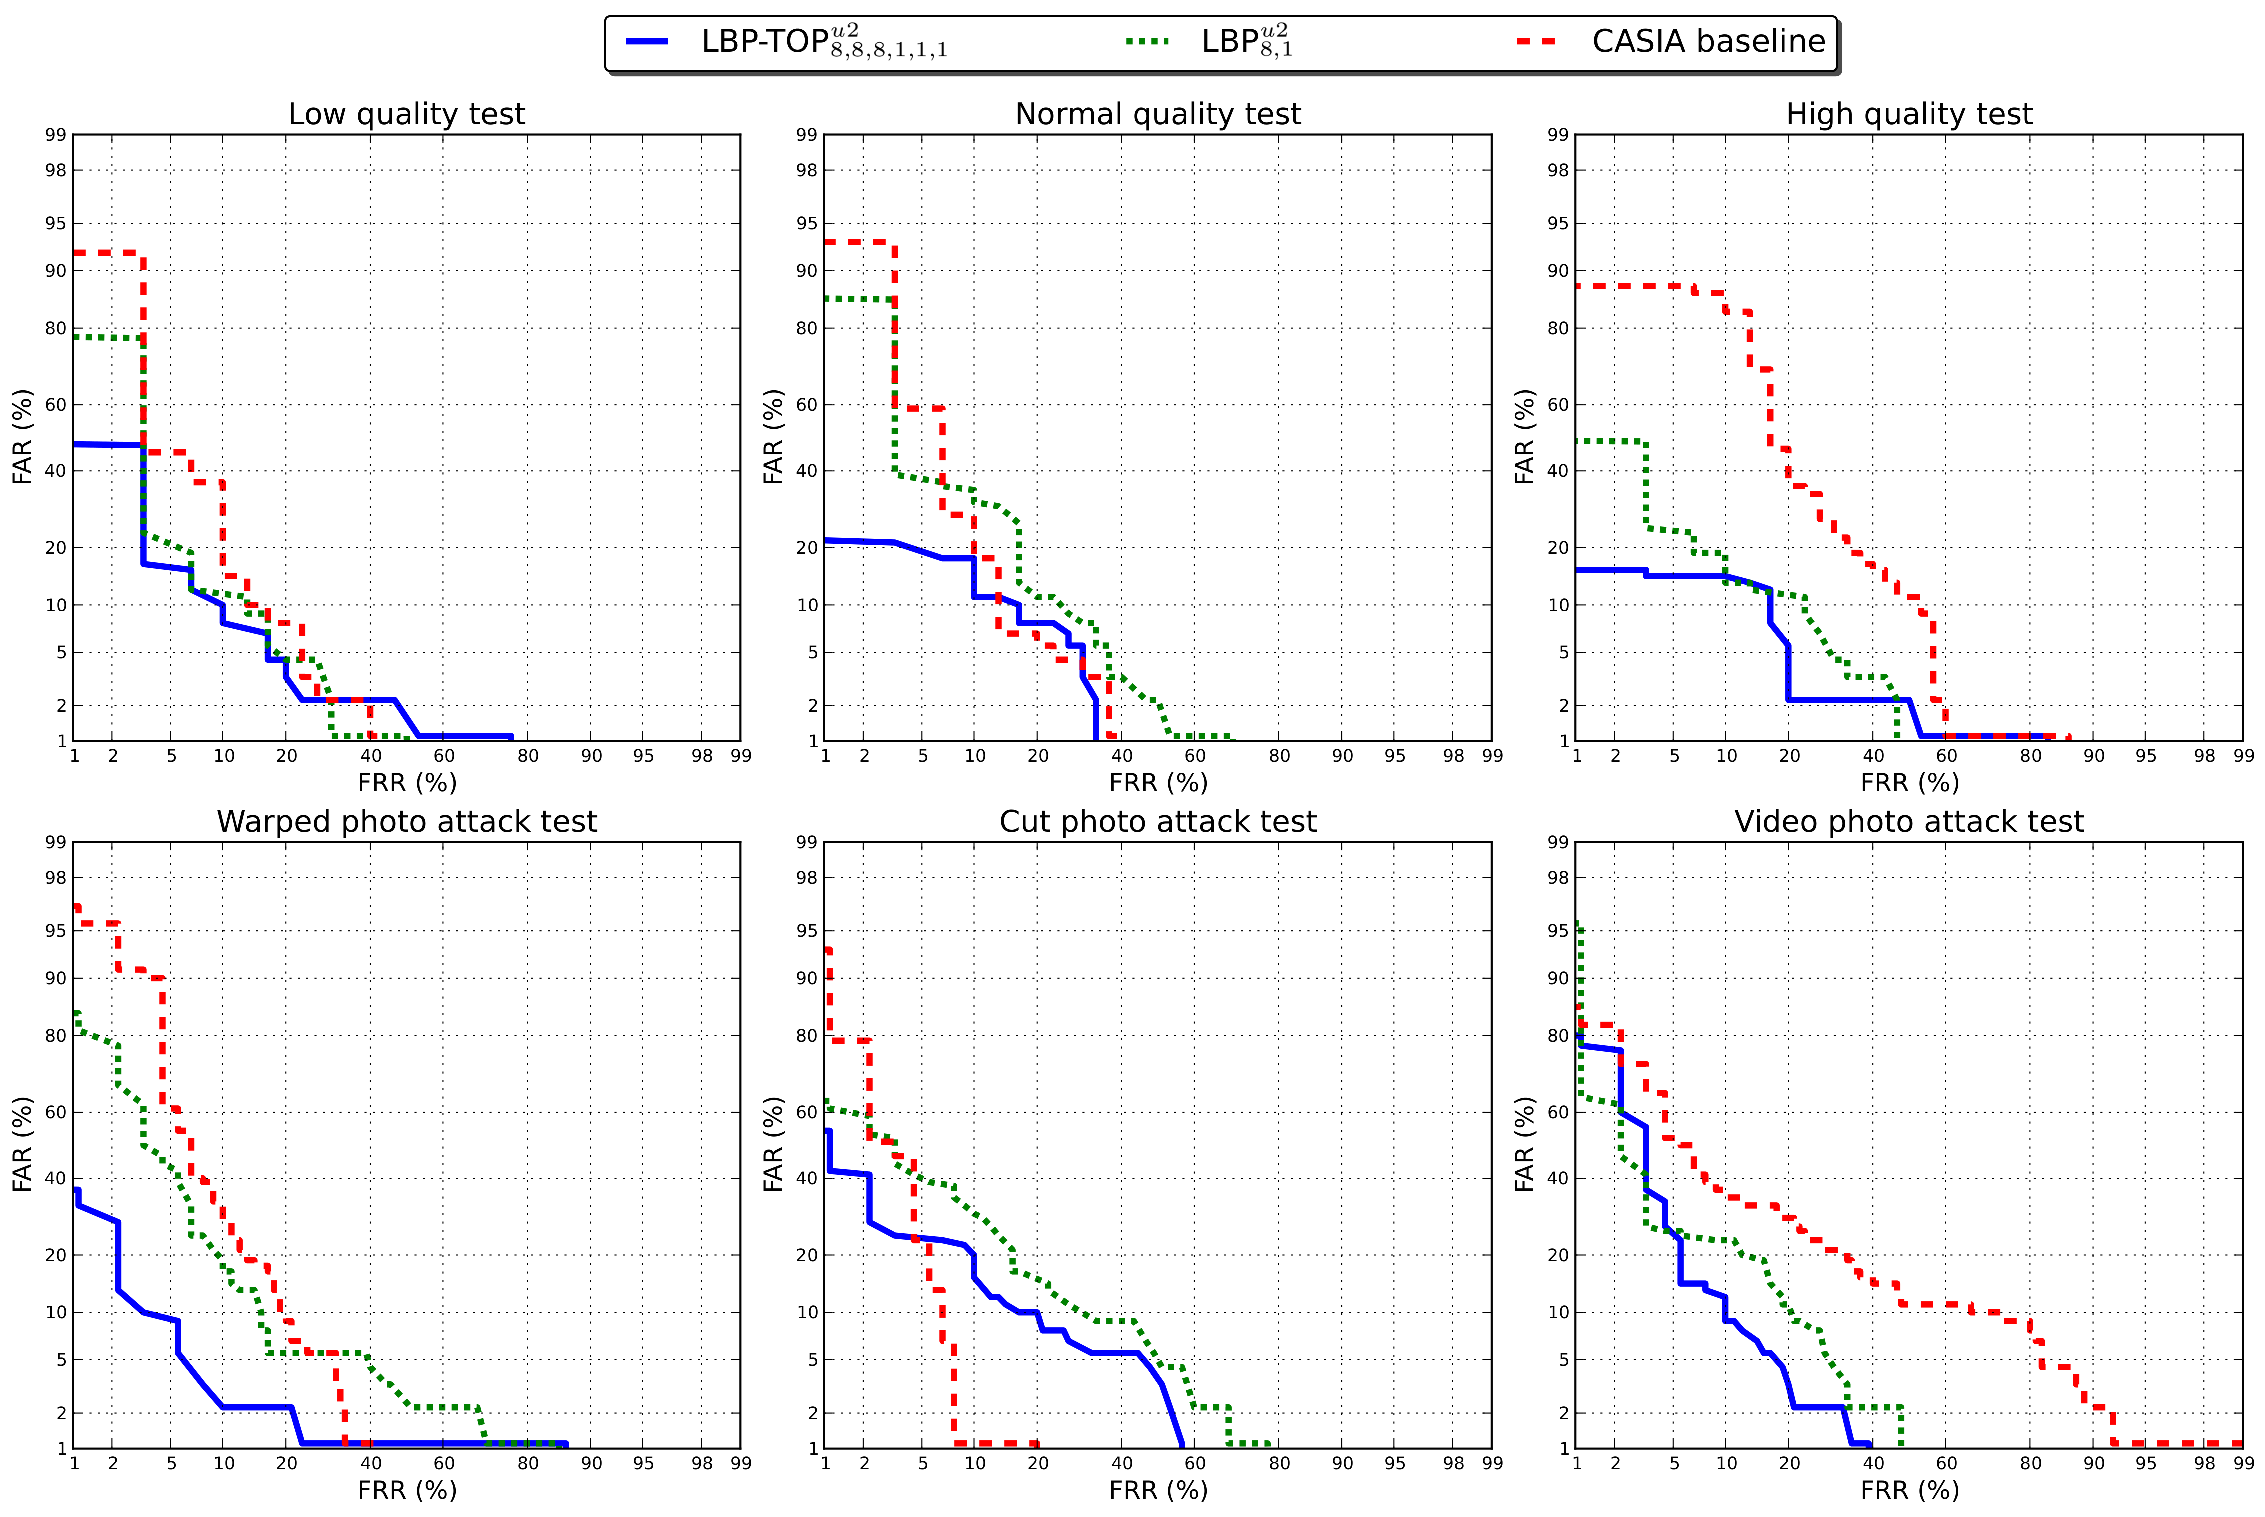
\includegraphics [width=\textwidth] {images/proposed_countermeasure/casia_overall_XYT_XY_baseline.pdf}
\caption[Performance of LBP-TOP$_{8,8,8,1,1,1}^{u2}$ using average of features compared to the DoG baseline method]{Performance of LBP-TOP$_{8,8,8,1,1,1}^{u2}$ using average of features compared to the DoG baseline method and LBP$_{8,1}^{u2}$ under the different protocols of the CASIA FASD. } \label{fig:DET_protocols}
\end{center}
\end{figure}

\begin{table}\centering
\caption{EER (in \%) development of LBP-TOP$_{8,8,8,1,1,1}^{u2}$ using average of features on the CASIA FASD.}
\begin{center}
\begin{tabular}{|c||c|c|c|c|c|c|}
\hline 
Frames & Low & Normal & High & Warped & Cut & Video \\
\hline 
{\centering 1} & {\centering 17} & {\centering 27} & {\centering 23} & {\centering 29} & {\centering 16} & {\centering 20} \\
\hline 
{\centering 5} & {\centering 13} & {\centering 20} & {\centering 20} & {\centering 19} & {\centering 14} & {\centering 14} \\
\hline 
{\centering 10} & {\centering 14} & {\centering 20} & {\centering 19} & {\centering 18} & {\centering 16} & {\centering 14}\\
\hline 
{\centering 25} & {\centering 13}& {\centering 13} & {\bf \centering 10} & {\centering 10} & {\centering 14} & {\centering 12} \\\hline 
{\centering 50} & {\centering 13}& {\bf \centering 11} & {\centering 10} & {\centering 7} & {\centering 13} & {\centering 10} \\
\hline 
{\centering 75} & {\bf \centering 10}& {\centering 12} & {\centering 13} & {\bf \centering 6}& {\bf \centering 12}& {\bf \centering 10} \\
\hline 
%{\bf \centering 0.13} & {\bf \centering 0.13} \\
\end{tabular}
\end{center}
\label{tab:eer_dev}
\end{table}

On the other hand, the spatiotemporal face description is able to improve the major drawbacks of DoG based countermeasure. Unlike the baseline method, our approach performs almost equally well at all three imaging qualities. Furthermore, the performance under warped photo and video attacks is significantly better. Especially the characteristic specular reflections (flickering) and excessive and distorted motion of warped photo attacks can be described very well.

%--------------------------------------------------------------------------------------------------------
\subsection{Discussion}
\label{sec:Proposed_summary}

Table \ref{tb_REPLAY_Results} and Table \ref{tb_CASIA_Results} summarize all the results obtained for each database following their provided protocols. In order to be comparable with still frame analysis presented for example in \cite{ChingovskaBIOSIG2012}, the results for Replay Attack Database represent the overall classification accuracy considering each frame individually. The access attempt based results are reported only for CASIA FASD as requested in its test protocol.

Table \ref{tb_REPLAY_Results} shows also the results for the LBP$^6$ \cite{ChingovskaBIOSIG2012} and the Motion Correlation$^7$ \cite{AnjosIJCB2011} based countermeasures whose source code is freely available. Table \ref{tb_CASIA_Results} contains the provided DoG based baseline and the holistic LBP based face description. It can be seen that the proposed countermeasure presented the best results overtaking the baseline results in both databases, thus confirming the benefits of encoding and exploiting not only the facial appearance but also the facial dynamics information. Unfortunately, our comparison is limited to these countermeasures due to the lack of publicly available implementations of other state-of-the-art techniques presented in literature. 

During these experiments we observed that the general performance of the proposed countermeasure was consistently better on Replay Attack Database compared to the CASIA FASD. As mentioned in Section \ref{sec_lbptop_planes}, the nature of the attack scenarios is different between the two datasets. In the Replay Attack Database, our LBP-TOP based face description was able to capture motion patterns of fixed photo attacks and scenic fake face attacks already when only relatively short time windows were explored. Performances below 10\% (HTER) were achieved. On the other hand, the CASIA FASD turned out to be more challenging from the dynamic texture point of view. Due to the lack of motion, analysis of longer temporal windows was required in order to find out distinctive motion patterns between genuine faces and fake ones. As it can be seen in Table \ref{tb_CASIA_Results}, by extending the micro-texture based spoofing detection into spatiotemporal domain, an improvement from 16\% to 10\% in terms of EER was obtained. The results also indicate that the proposed dynamic texture based face liveness description was able to improve the state of the art on both datasets.


\begin{table}
   \caption{HTER(\%) of the best results achieved on the Replay Attack Database (following the database protocol) comparing with the provided baseline.}
   \begin{center}

     \begin{tabular}{l | c c | c c |}
        \cline{2-3}
         & \textbf{dev} & \textbf{test} \\ \hline
         \multicolumn{1}{|l|}{Motion Correlation \cite{AnjosIJCB2011} } & 11.78 & 11.79  \\ \hline
         \multicolumn{1}{|l|}{LBP$_{8,1}^{u2}$ + SVM} & 14.84 & 15.16 \\ \hline
         \multicolumn{1}{|l|}{LBP$_{3\times3}$ + SVM~\cite{ChingovskaBIOSIG2012}} & 13.90 & 13.87 \\ \hline         
        \multicolumn{1}{|l|}{LBP-TOP$^{u2}_{8,8,8,1,1,1}$ + SVM} & 8.17 & 8.51  \\ \hline
        \multicolumn{1}{|l|}{LBP-TOP$_{8,8,8,1,1,[1-2]}$ + SVM} & 7.88 & 7.60  \\ \hline
     \end{tabular}
   \end{center}
   \label{tb_REPLAY_Results}
\end{table}

\begin{table}
   \caption{$EER(\%)$ of the best results achieved on the CASIA FASD (following the database protocol) comparing with the provided baseline.}
   \begin{center}

     \begin{tabular}{l | c |}
         \cline{2-2}
         & \textbf{test} \\ \hline
         \multicolumn{1}{|l|}{DoG baseline \cite{zhangface}} & 17 \\ \hline
         \multicolumn{1}{|l|}{LBP$_{8,1}^{u2}$ + SVM} & 16 \\ \hline
         %\multicolumn{1}{|l|}{LBP$_{3\times3}$~\cite{ChingovskaBIOSIG2012,maatta2011face}} & 16 \\ \hline
         \multicolumn{1}{|l|}{LBP-TOP$^{u2}_{8,8,8,1,1,1}$ with average of features + SVM} & 10  \\ \hline
         %\multicolumn{1}{|l|}{LBP-TOP$_{8,8,8,1,1,[1-2]}$ with average of features + SVM} & \textbf{9}  \\ \hline

     \end{tabular}
   \end{center}
   \label{tb_CASIA_Results}
\end{table}

%%%%%%%%%%%%%%%%%%%%%%
%%%%%%%%%%%%%%%%%%%%%%
% Conclusion
%%%%%%%%%%%%%%%%%%%%%%
%%%%%%%%%%%%%%%%%%%%%%

\section{Final Remarks}
\label{sec:Proposed_finalremarks}

Inspired by the recent progress in dynamic texture, the problem of face spoofing detection was investigated in this chapter using spatiotemporal local binary patterns. The key idea of the proposed countermeasures consists of analysing the structure and the dynamics of the micro-textures in the facial regions using $LBP-TOP$ features that provides an efficient and compact representation for face liveness description. The experiments carried out with this countermeasure consistently outperform prior works on both datasets. Best results were achieved using nonlinear SVM classifier but it is important to notice that experiments with simpler LDA based classification scheme resulted in comparable performance under various spoofing attack scenarios. Thus, the use of simple and computationally efficient classifiers should be indeed considered when constructing real-world anti-spoofing solutions. The results presented in this chapter is reproducible. The source code with instructions on how to reproduce the results is freely available\footnote{\url{https://pypi.python.org/pypi/antispoofing.lbptop/}}.


%\chapter{The Comparative Study}
\label{chap:Comparative_Study}

This chapter provides the gui


This chapter provides the experiments and the results of this comparative study of countermeasures. As aforementioned in the last chapter, four countermeasures were selected and each one deal with one of the main cues mentioned in Section \ref{sec:SpoofingAttacksFaceRec} (liveness detection, scene characteristics and differences in image quality assessment). The countermeasures are:



\section{Evaluated countermeasures}
\label{sec:Evaluated_countermeasures}

For this comparative study were selected four countermeasures that do not depend of the user collaboration. Very representative according to the state of the art in the face antispoofing research, each one explore one of the main cues mentioned in the\ref{sec:SpoofingAttacksFaceRec}. Next subsections presents the details of each countermeasure and how was set each hyper-parameters of each one.

\subsection{Motion Correlation}

As presented in Section \ref{sec:scene_cues}, the Motion correlation \cite{AnjosIJCB2011} countermeasure measures the correlation between the face and it background. With some contributions by our side, the source code of this countermeasure is freely available \footnote{https://github.com/bioidiap/antispoofing.motion/}. There are, basically, two hyper-parameters in this countermeasure. The first one is the number of frames used to compute the 5 quantities. The second one is the binary classifier.

As the authors suggested, twenty frames to compute the 5 quantities are sufficient to the algorithm converge in their experiments. The classifier suggested in the paper was one based on Multi-layer Perceptron. This classifier has, basically, the number of hidden layers and the number neurons in each hidden layer as hyper-parameters. The authors suggested one hidden layer and five neurons in this hidden layer as good tradeoff between computational complexity and performance. 

\subsection{Textures with $LBP$}

Presented in Section \ref{sec:quality_assessment}, the countermeasure based on Textures with $LBP$ \cite{ChingovskaBIOSIG2012} and \cite{maatta2011face} explore the differences in texture properties between real accesses and attacks in single frames. 

There are, basically, three hyper-parameters in this countermeasure. The first one is the geometrically normalized face size. The authors suggested a face size of $64 \times 64$ pixels. The second one is the configuration of the $LBP$ texture descriptor. The $LBP$ itself has several hyper-parameters \ref{inen2011computer} and the authors of both papers stressed only some of that. In this thesis we will follow the setup suggested by \cite{ChingovskaBIOSIG2012} using the $LBP_{8,1}^{u2}$. Finally the last hyper-parameter is the binary classifier. The best classifier tested by \cite{ChingovskaBIOSIG2012} was the Support Vector Machines (SVM) using the Radial Basis Function (RBF). For this classifier the parameter $C$ (the cost of the loss function) and the $\gamma$ parameter (the variance of the radial function) was set to $1$ and $0.1$ respectively.

\subsection{Dynamic Textures with $LBP-TOP$}

Presented in the Chapter \ref{chap:Proposed_Countermeasures}, the countermeasure based on dynamic textures with $LBP-TOP$, explore the texture dynamics to detect attacks in a frame sequence. There are, basically, three hyper-parameters in this countermeasure. The first one is the geometrically normalized face size. In the last chapter, we worked with face sizes of $64 \times 64$ pixels and we are keep this in the next experiments. The second hyper-parameter is the configuration of the $LBP-TOP$ descriptor. As in the $LBP$, the $LBP-TOP$ descriptor itself has several hyper-parameters and each one was extensively tuned in the last chapter. As good tradeoff between computational complexity and performance we selected the following configuration: $LBP-TOP^{u2}_{8,8,8,1,1,1}$. The last hyper-parameter is the binary classifier. The evaluation method proposed in the last chapter suggested the SVM classifier with RBF kernel.


\subsection{Eye blinks}

The eye blink countermeasure used in this thesis uses a similar technique applied in Motion Correlation countermeasure\cite{AnjosIJCB2011}. The difference is; the accumulated motion $M_D$, (see Equation \ref{eq:motion}) is computed between the face region and the eyes region as can be observed in the Figure \ref{fig:eye_blink}. 

\begin{figure}[!btb]
\begin{center}
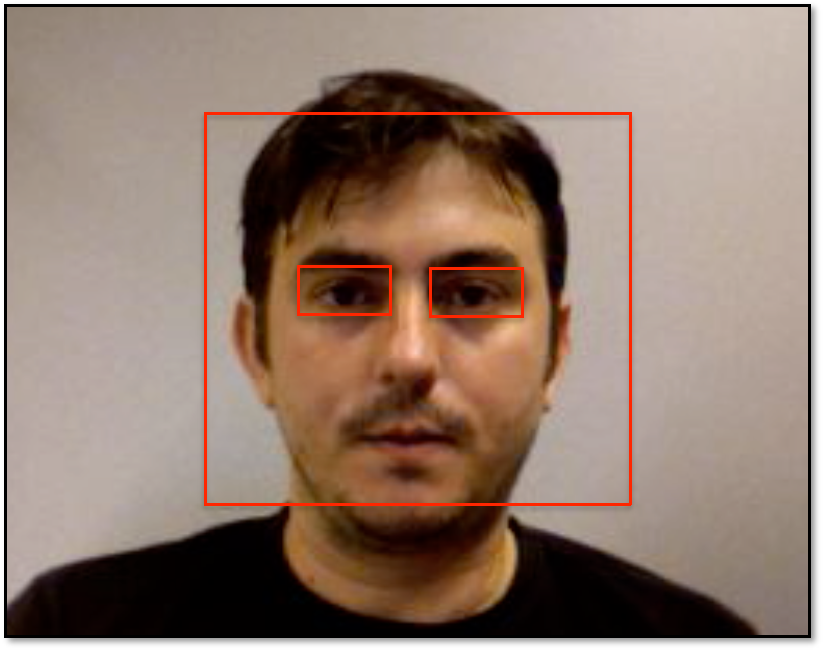
\includegraphics [width=10cm] {images/eye_blink.pdf}
\caption[Eye blink countermeasure scheme]{Eye blink countermeasure scheme}
\label{fig:eye_blink}
\end{center}
\end{figure}


The score for each single frame $n$ in a frame sequence, is computed using the following equation:
\begin{equation}
S_n=   \frac{M_{D_{eye}}(n)}{M_{D_{face}}(n)} - ravg(\frac{M_{D_{eye}}}{M_{D_{face}}})(n)
\label{eq:score_blink}
\end{equation}
where the $ravg$ is the remainder average in a frame sequence until the frame $n$.


\section{Evaluation method}
\label{sec:Evaluation_Protocol}

For this comparative study, we will evaluate the intra-database and the inter-database (or cross-database) generalization. For that, we developed two test protocols, the intra-test protocol and the inter-test protocol. 

The intra-test protocol evaluates the intra-database generalization. It consists in training, tuning and testing a countermeasure with the respectively training set, development set and test set of one database.

The inter-test protocol is a little bit more challenging since test the inter-database generalization (or cross-database). It consists in training and tuning a countermeasure with the training set and development set of one database and test it with the test set of others databases. 


%Firstly, we study how the countermeasures, presented in Section \ref{sec:countermeasures}, will perform in a more realistic condition. This condition consists in training and tuning each one of the countermeasures with one face anti-spoofing database and testing with another one. To report the performance in such a scenario, two evaluation protocols were designed to work with the databases described in Section \ref{sec_replay}. These protocols are the "intra-test" protocol and the "inter-test" protocol.


%The inter-test protocol evaluates the countermeasure performance in a more realistic scenario, close to real usage conditions. It consists in training and tuning a countermeasure with the training set and development set of one database and test it with the test set of another one. With this protocol, it is possible to evaluate the performance and the generalization power of a countermeasure in a set of unseen types of attacks.


\section{Evaluation Metrics}

The final performance of each countermeasure using both evaluation protocols in the test set of each database is reported with the Half Total Error Rate ($HTER$): 

\begin{equation}
\label{eq:HTER}
HTER(D_2)=\frac{FAR(\tau(D_1),D_2)+ FRR(\tau(D_1),D_2)} {2} ,
\end{equation}
where $\tau(D_n)$ is the decision threshold, $D_n$ is the dataset, $FAR$ is the False Acceptance Rate in the database $D_2$ and $FRR$ is the False Rejection Rate in the database $D_2$. In this protocol, the value of $\tau(D_n)$ is estimated on the Equal Error Rate (EER) using the development set of the database $D_1$. 

In this equation, to measure the performance using the intra-database protocol, is necessary to consider $D_1 = D_2$. To measure the performance using the inter-database protocol, is necessary to make $D_1 \neq D_2$.


\section{Evaluated data}

As the Motion correlation, $LBP-TOP$ and the eye blink countermeasures need a frame sequence to work, the databases evaluated in this dissertation will be the Replay Attack Database (Section \ref{sec_replay}) and CASIA Face Antispoofing Database (Section \ref{sec_casia}).

As already mentioned in Section \ref{sec_replay} the Replay Attack Database has three non-overlapping partitions; the training, development and test set for respectively train, tune and test a countermeasure. To run the proposed protocols in this database, we will used the train set to train the four countermeasures; the development set will be used to estimate the value of $\tau(D_1)$. Finally the test set will be used to report the $HTER(D_2)$.

The CASIA FASD lacks a specific development set; this database has only a train and a test set. Since we need the three sets (train, development and test), we split the train set in five partitions and a 5-fold cross-validation training was done. For that, 4 folds were used for training and 1 fold was used to estimate the value of $\tau(D_1)$. The original test set was preserved, to report the $HTER(D_2)$. Because of 5-fold cross validation protocol, for the CASIA FASD 5 results were generated. The average of $HTER$ was provided as a final result.



\chapter{Experiments and Results}
\label{chap:Experiments_Results}

This chapter provides the experiments results of this comparative study of countermeasures. Three countermeasures were selected for this study:
\begin{itemize}
        \item Dynamic textures with $LBP-TOP$;
        \item Textures with $LBP$ (\cite{ChingovskaBIOSIG2012} and \cite{maatta2011face});
        \item Motion correlation (\cite{AnjosIJCB2011}).
\end{itemize}
As the Motion correlation and $LBP-TOP$ countermeasures need a frame sequence to work, the databases evaluated in this work were the Replay Attack Database (Section \ref{sec_replay}) and CASIA Face Antispoofing Database (Section \ref{sec_casia}).

The Section \ref{sec:Intra_test} compare the countermeasures in the Intra-test protocol. Section \ref{sec:Inter_test} compare the countermeasures in the Inter-test protocol. In the Section \ref{sec:combination} the combination of databases is explored to train each one of the countermeasures. In Section \ref{sec:framework} the Score Level Fusion based Framework is explored to train each countermeasure. Finally Section \ref{sec:Summary} sumarizes the experiments.

\section{Intra-test protocol}
\label{sec:Intra_test}

Table \ref{tb:IntraTest} shows the performance of the three countermeasures, in HTER terms, applying the Intra-test protocol.

\hspace{-17mm}\begin{table}[ht!]
\caption{$HTER(\%)$ of each countermeasure applying the intra-test ($D_1=D_2$) protocol.}
\begin{center}
  \begin{tabular}{ | c | c | c | c  c | }
    \hline

   \multirow{2}{*}{\textbf{Countermeasure}} & \textbf{Train/Tune} & \textbf{Test} & \multicolumn{2}{c|}{\textbf{HTER(\%)}} \\ 
     & $D_1$ & $D_2$ & \textbf{dev} & \textbf{test}  \\ \hline
    
    \multirow{2}{*}{Correlation} & Replay  & Replay  &  11.66 & 11.79 \\ 
               & CASIA &  CASIA  & 24.91 & 31.36 \\ \hline \hline

    \multirow{2}{*}{$LBPTOP_{8,8,8,1,1,1}^{u2}$}  & Replay & Replay  & 8.17 & 8.51  \\
               & CASIA  & CASIA  & 21.77 & 22.27 \\ \hline \hline

    \multirow{2}{*}{$LBP_{8,1}^{u2}$} & Replay  & Replay  & 14.41 &15.45  \\
               & CASIA  & CASIA  & 23.00  & 22.54 \\
            
    \hline
  \end{tabular}
\end{center}
\label{tb:IntraTest}
\end{table}

Analyzing the performance in the intra-test protocol ($D_1 = D_2$) it can be observed that different countermeasures have different performances in different databases. However, it is possible to observe a that all the three countermeasures have a good overall performance and a good intra-database generalization power. The good generalization performance can be attested comparing the results between the development set and the test set. In Table \ref{tb:IntraTest} the $HTER(\%)$ in the development set and the $HTER(\%)$ in the test set are very similar. In Figure \ref{fig:ROC_cross} the ROC curves blue and red (dashed line and solid line) represents the intra-test test protocol. It can be observed that the curves are almost overlapped.


\section{Inter-test protocol}
\label{sec:Intra_test}

Table \ref{tb:InterTest} shows the performance of the three countermeasures, in HTER terms, applying the Inter-test protocol.

\hspace{-17mm}\begin{table}[ht!]
\caption{$HTER(\%)$ of each countermeasure applying the inter-test ($D_1 \neq D_2$) protocol.}
\begin{center}
  \begin{tabular}{ | c | c | c | c  c | }
    \hline

   \multirow{2}{*}{\textbf{Countermeasure}} & \textbf{Train/Tune} & \textbf{Test} & \multicolumn{2}{c|}{\textbf{HTER(\%)}} \\ 
     & $D_1$ & $D_2$ & \textbf{dev} & \textbf{test}  \\ \hline
    
    \multirow{2}{*}{Correlation} &  Replay & CASIA & 11.66 & 61.78  \\ 
               & CASIA  & Replay & 24.91 & 48.47  \\ \hline \hline

    \multirow{2}{*}{$LBPTOP_{8,8,8,1,1,1}^{u2}$}  &  Replay  & CASIA  & 8.17 & 51.05   \\
               & CASIA  & Replay & 21.77 & 61.11   \\ \hline \hline

    \multirow{2}{*}{$LBP_{8,1}^{u2}$} &  Replay  & CASIA  & 46.87  & 48.06   \\
               & CASIA  & Replay & 23.00 & 57.64  \\
            
    \hline
  \end{tabular}
\end{center}
\label{tb:InterTest}
\end{table}

Analyzing the performance in the inter-test protocol ($D_1 \neq D_2$), it can be observed that the performance results considerably degrade compared with the intra-test protocol and it becomes evident that both databases and the methods are strongly biased indicating the countermeasures do not generalize as expected. In Table \ref{tb:InterTest} the $HTER(\%)$ in the development set and the $HTER(\%)$ in the test set are quite different. In Figure \ref{fig:ROC_cross} the ROC curves blue and green (dotted line and solid line) represents the inter-test test protocol. It can be observed that the curves are quite distant from each other.

The results indicate that the countermeasures and the databases introduce some bias on the spoofing detections. The countermeasures bias are possibly related to the feature selection. The databases bias are possibly related with the types and styles of attacks that is hard to generalize. In next experiment, we stray if the countermeasures are truly biased to databases or can be tuned to overcome the database bias.

\begin{figure*}[ht]
\begin{center}
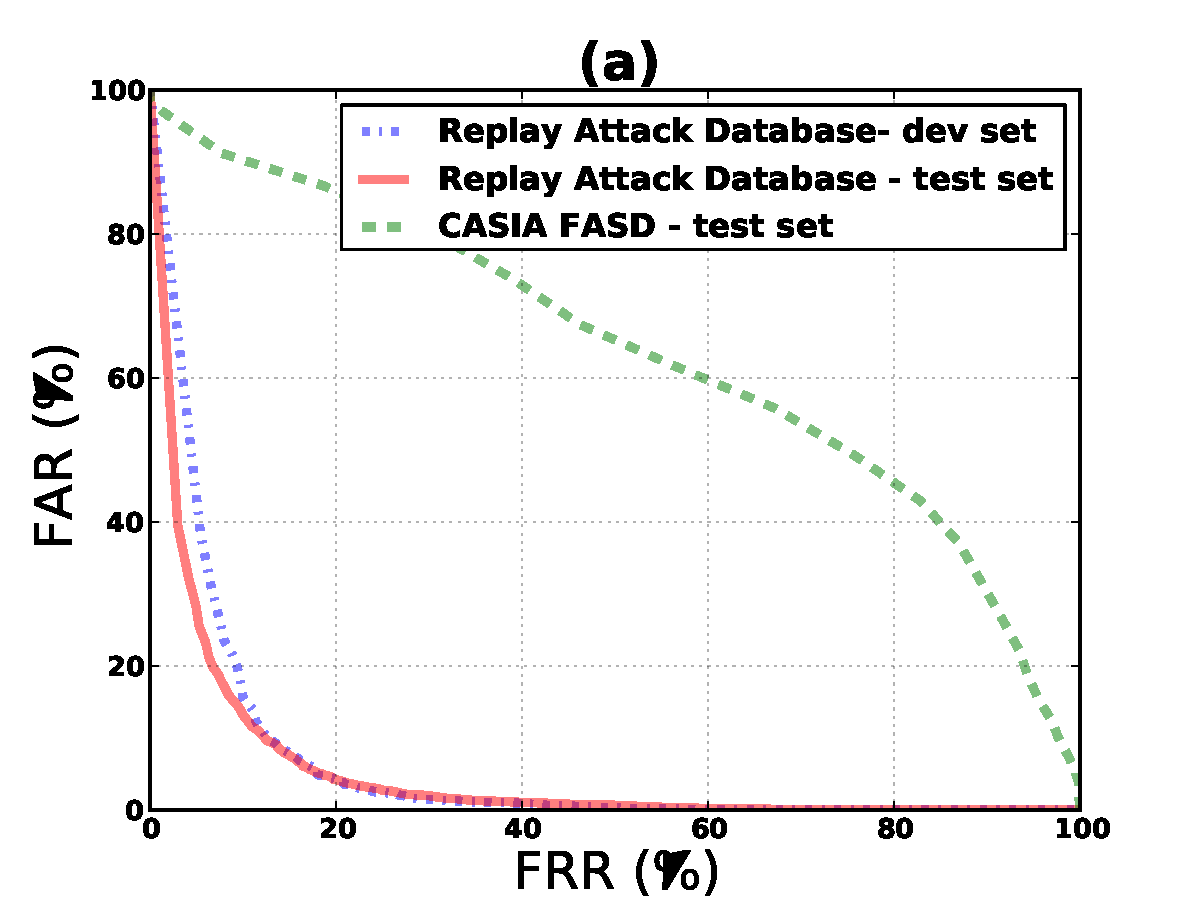
\includegraphics [width=5cm] {plots/CROSS-DATABASE/MOTION/roc_replay-machine.pdf} 
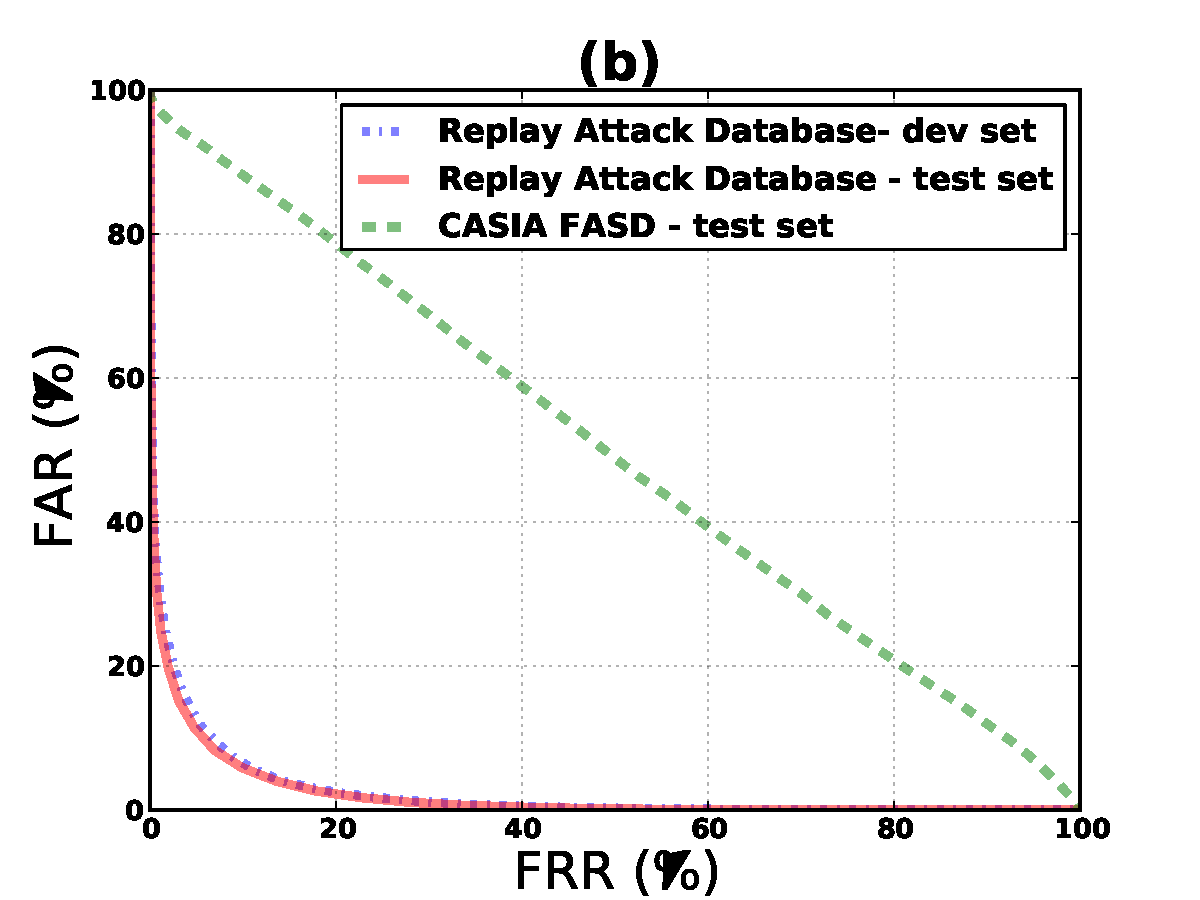
\includegraphics [width=5cm] {plots/CROSS-DATABASE/LBPTOP/roc_replay-machine.pdf}
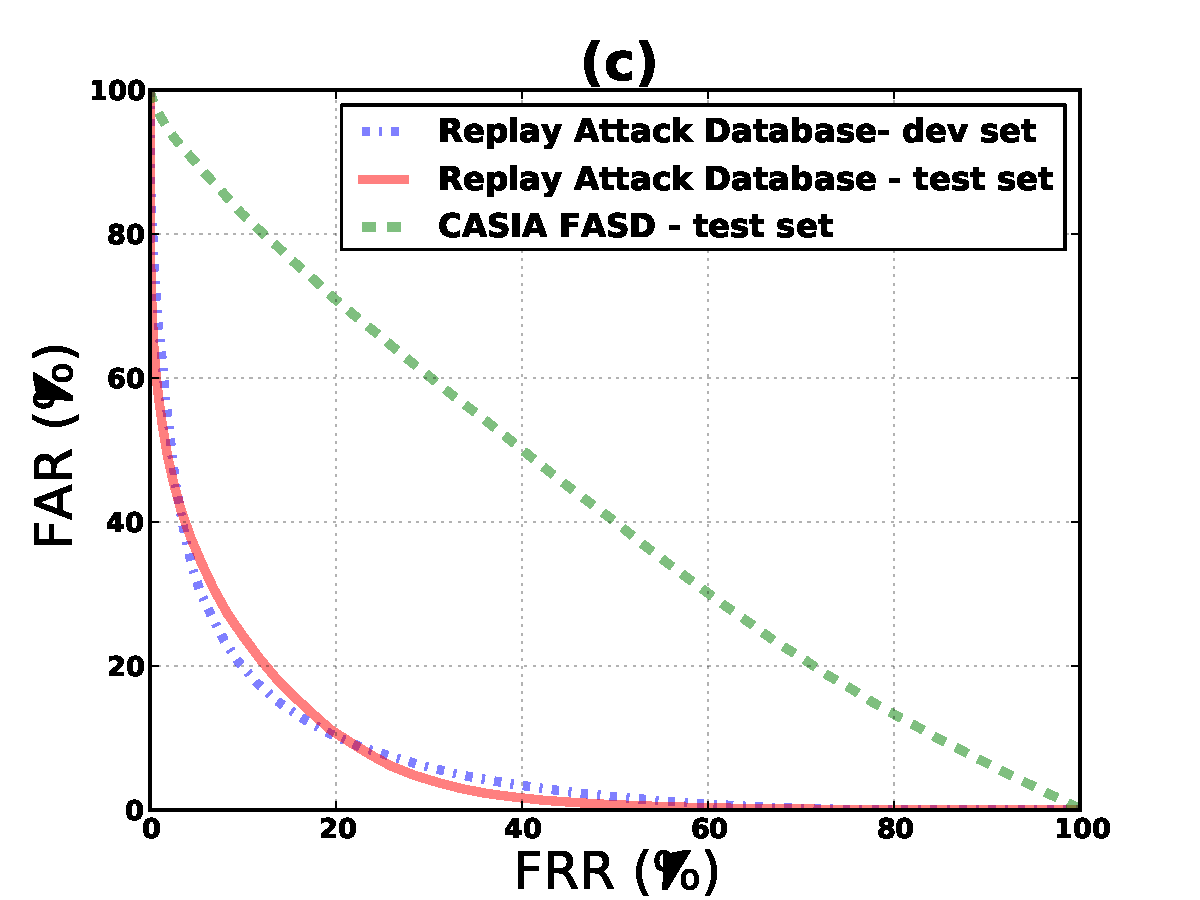
\includegraphics [width=5cm] {plots/CROSS-DATABASE/LBP/roc_replay-machine.pdf}

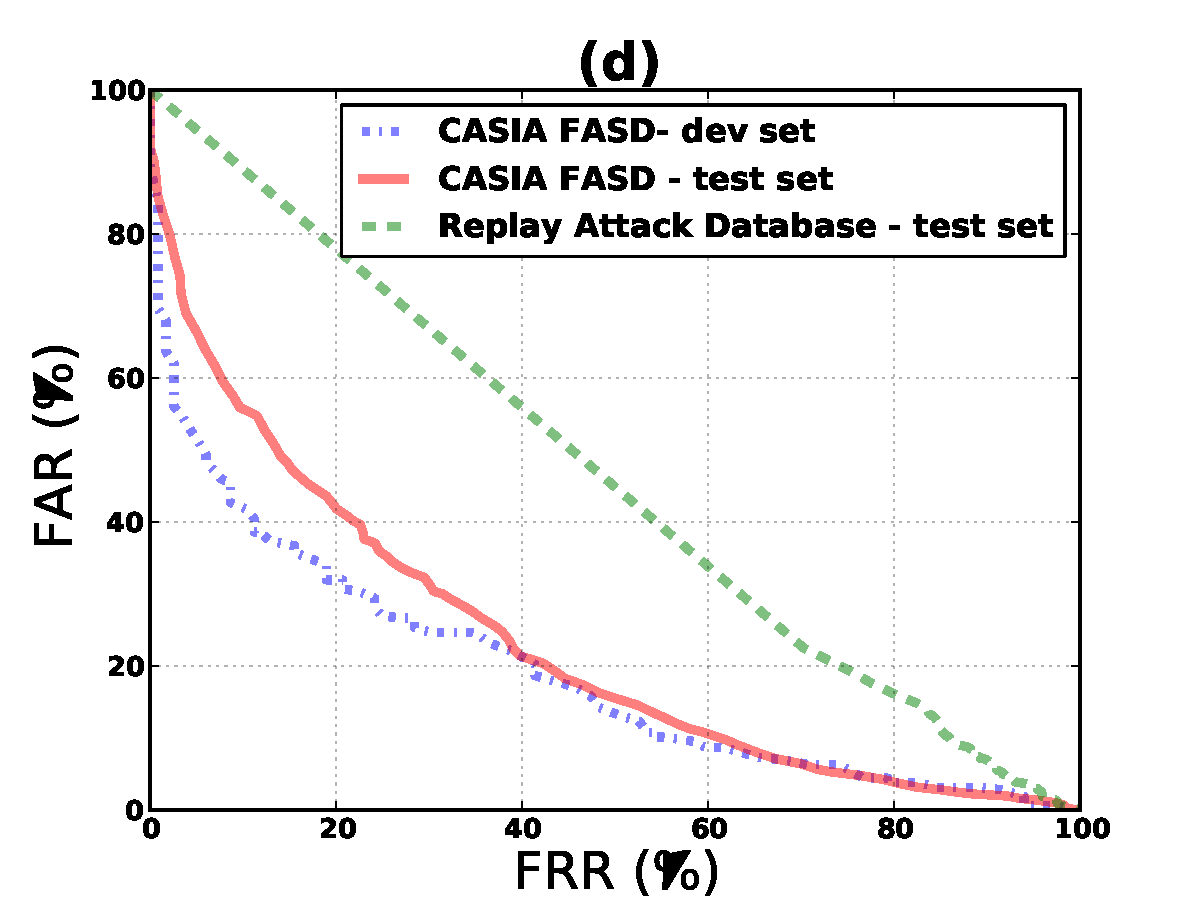
\includegraphics [width=5cm] {plots/CROSS-DATABASE/MOTION/roc_casia_fasd-machine.pdf} 
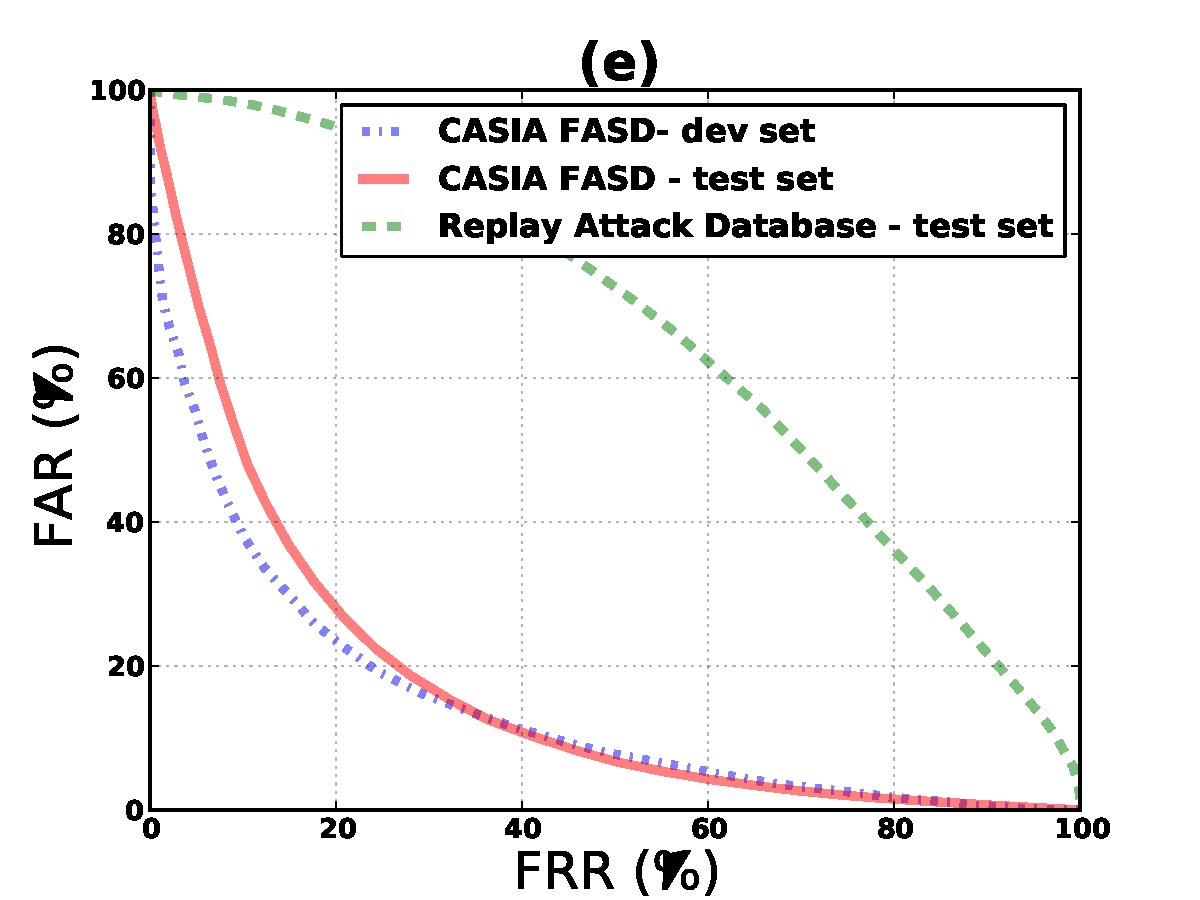
\includegraphics [width=5cm] {plots/CROSS-DATABASE/LBPTOP/roc_casia_fasd-machine.pdf}
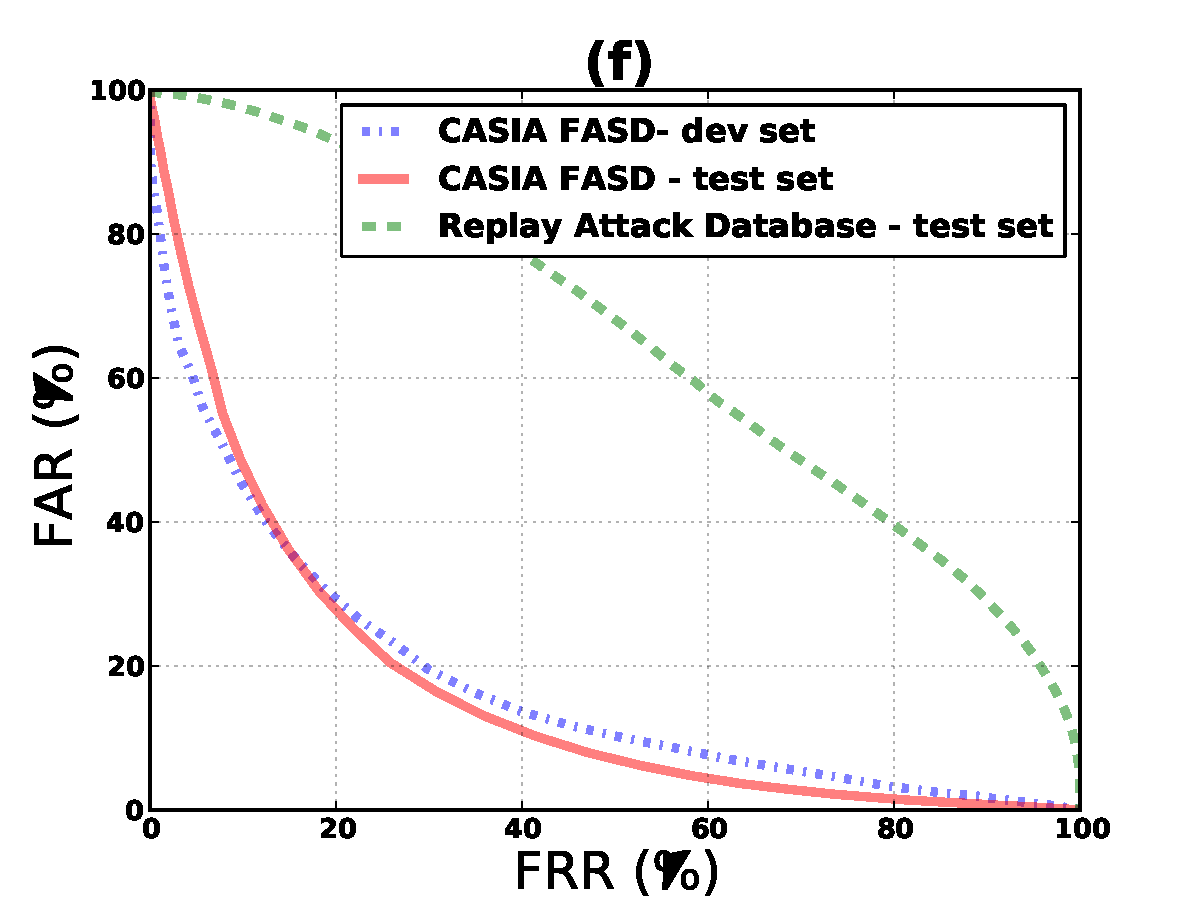
\includegraphics [width=5cm] {plots/CROSS-DATABASE/LBP/roc_casia_fasd-machine.pdf}

\caption{ROC curves of each countermeasure using the intra-test and the inter-test protocol. (a) Correlation with frame differences countermeasure trained and tuned with the Replay Attack Database (b) $LBP-TOP$ countermeasure trained and tuned with the Replay Attack Database (c) $LBP$ countermeasure trained and tuned with the Replay Attack Database (d) Correlation with frame differences countermeasure trained and tuned with the CASIA-FASD (e) $LBP-TOP$ countermeasure trained and tuned with the CASIA-FASD (f) $LBP$ countermeasure trained and tuned with the CASIA-FASD.} 
\label{fig:ROC_cross}
\end{center}
\end{figure*}


\section{Combination of Multiple Databases}
\label{sec:combination}

Say something.

%Analyzing the performances with this strategy compared with the performance obtained with the inter-set protocol, can be observed a significant improvement for all countermeasures ($\sim41.9\%$ in HTER average improvement). However, comparing with the intra-test protocol the performance drops drastically ($\sim64\%$ in HTER average degradation). It can be observed that the performance for CASIA FASD degrades more than for the Replay Attack Database suggesting a strong bias for this database. The Replay Attack Database has twice more data than the CASIA FASD, and this difference is biasing the final performance.

%This strategy also has one drawback: when a new database with new types of attacks needs to be added, it is necessary to train and tune all the countermeasures again.


\begin{table}[ht]
\caption{$HTER(\%)$  of each countermeasure trained with Replay Attack Database and CASIA FASD and test it with each test set of each database.}
\begin{center}
  \begin{tabular}{ | c | c | c  c |}
    \hline

   \multirow{2}{*}{\textbf{Countermeasure}} &  \multirow{2}{*}{\textbf{Test}} & \multicolumn{2}{c|}{\textbf{HTER(\%)}} \\ 
    &&\textbf{dev} & \textbf{test}  \\ \hline
    
    \multirow{2}{*}{Correlation} & Replay  &  \multirow{2}{*}{12.18} & 24.14 \\ 
               & CASIA &  & 43.30  \\ \hline \hline

    \multirow{2}{*}{$LBPTOP_{8,8,8,1,1,1}^{u2}$}  & Replay  & \multirow{2}{*}{14.29} & 10.67 \\
               &  CASIA  & & 42.04  \\ \hline \hline

    \multirow{2}{*}{$LBP_{8,1}^{u2}$}  & Replay  & \multirow{2}{*}{20.45} &19.07 \\
                & CASIA  &  & 45.92 \\
    \hline
  \end{tabular}
\end{center}
\label{tb:TrainAllTest}
\end{table}


\begin{figure}[ht]
\begin{center}

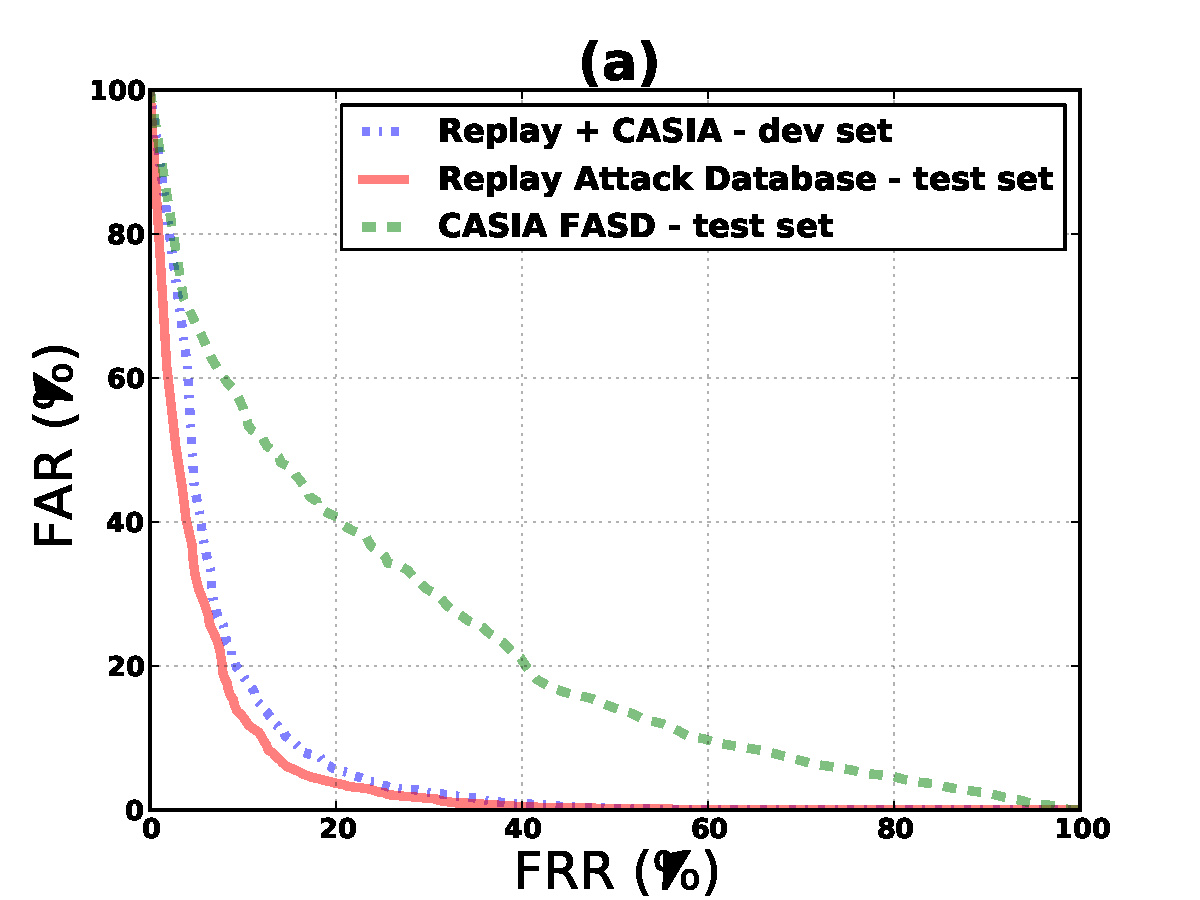
\includegraphics [width=5.5cm] {plots/ALL/MOTION.pdf} 
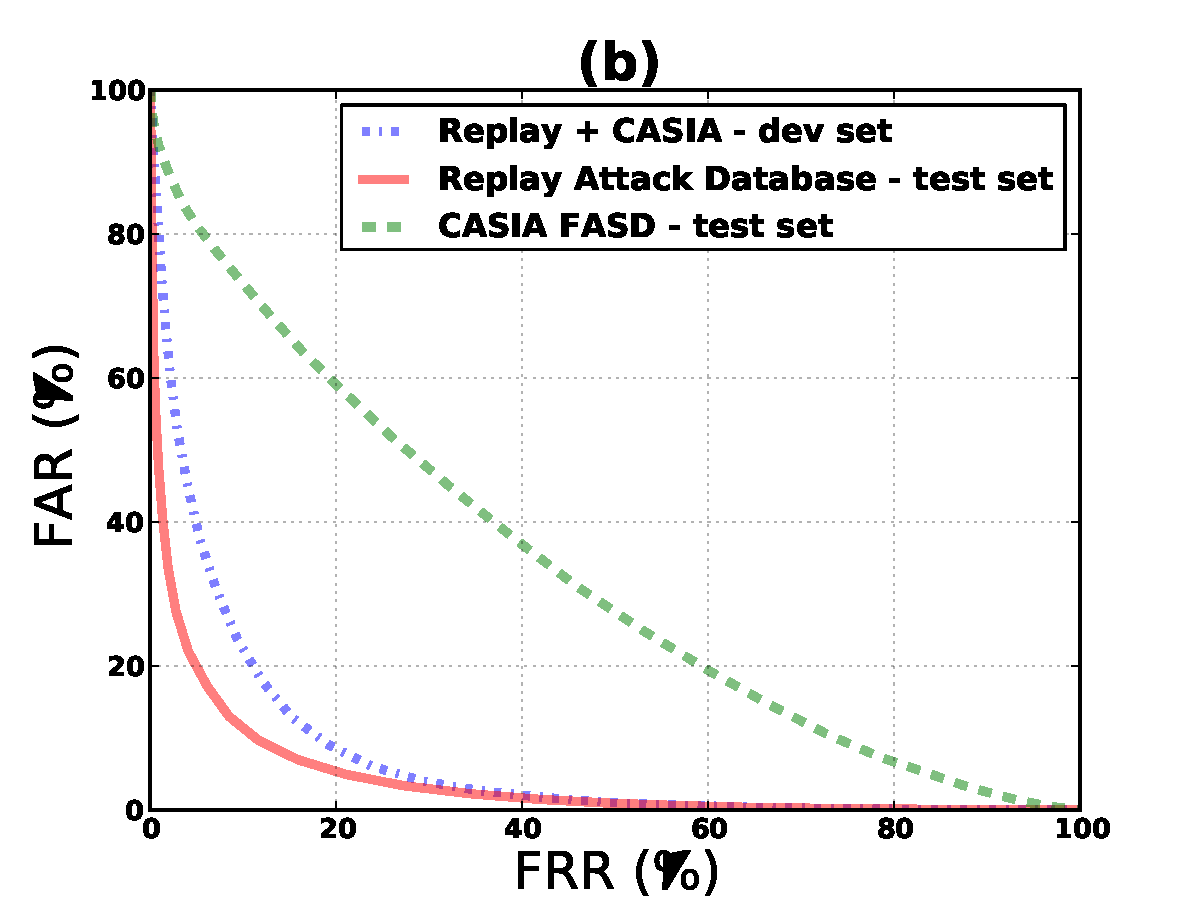
\includegraphics [width=5.5cm] {plots/ALL/LBPTOP.pdf}
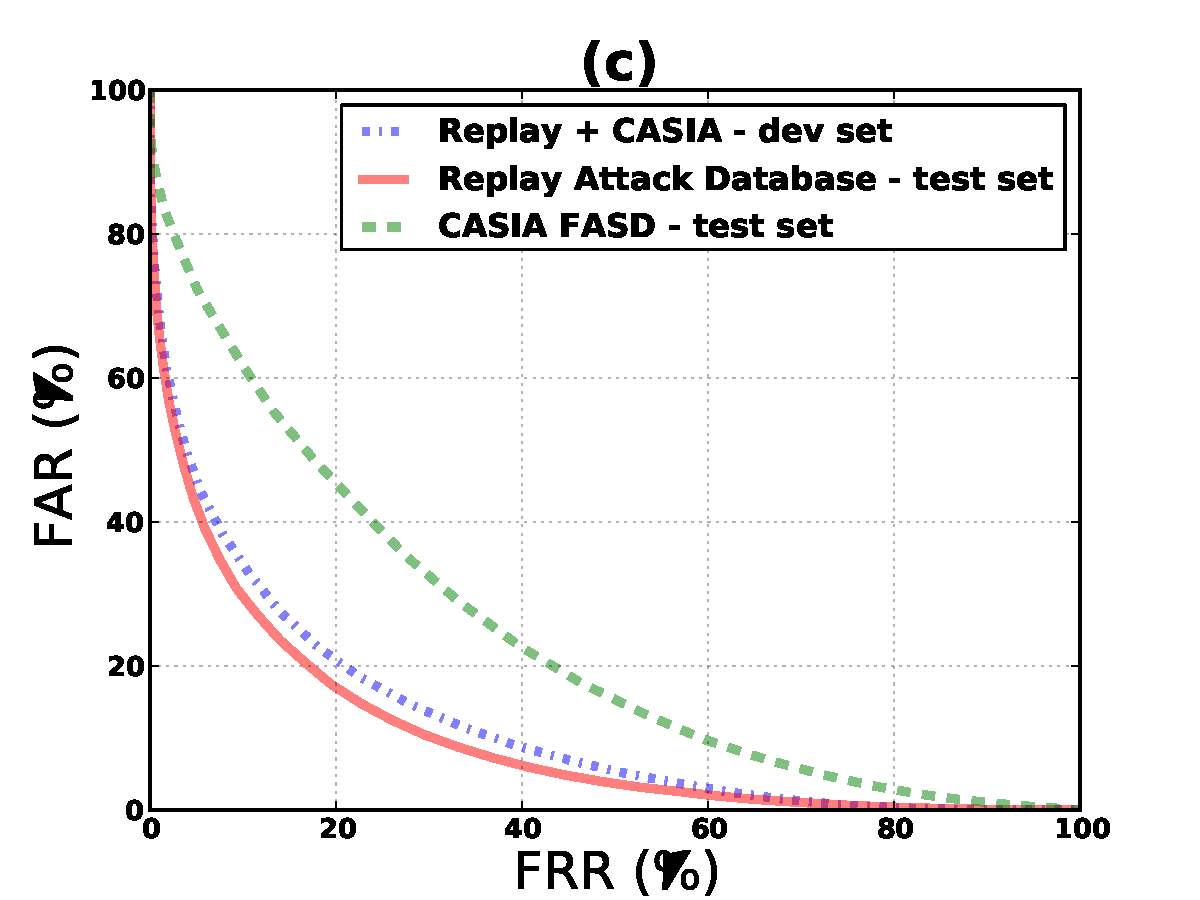
\includegraphics [width=5.5cm] {plots/ALL/LBP.pdf}

\caption{ROC curves of each countermeasure trained with Replay Attack Database and CASIA FASD and test it with each test set of each database. (a) Correlation with frame differences (b) $LBP-TOP$ countermeasure (c) $LBP$ countermeasure} 
\label{fig:ROC_cross}
\end{center}
\end{figure}


\section{Score Level Fusion based Framework}
\label{sec:framework}

To improve the performance results in comparison with the intra-test protocol and the inter-test protocol and to mitigate the bias mentioned in the last section, we introduce a framework based on score level fusion. Using this framework, when a new countermeasure need to be added, it is possible to "plug it" without any extra training steps required for the other countermeasures.

To support this assumption, we first evaluate the level of independence of the countermeasures trained with different databases in order to ensure its effectiveness in a possible score fusion. Kulcheva and Whitaker \cite{kuncheva2003measures} show that the combination of statistically independent classifiers is a recommended for a good performance in a score level fusion. In order to evaluate the dependence of classifiers, ten statistics were analyzed. The methodology presented on that work shows that the $Q-statistic$ is most suitable and we choose that metric to evaluate the statistic dependence of each countermeasure for the Score Level Fusion based Framework. The $Q-statistic$ for two classifiers is defined as follow:

\begin{equation}
\label{eq:Qstatistic}
Q_{R,C} = \frac{N_{11}N_{00} - N_{01}N_{10}}{N_{11}N_{00} +N_{01}N_{10}}
\end{equation}
where $R$ is the countermeasure trained with the Replay Attack Database; $C$ is the countermeasure trained with CASIA FASD; $N_{11}$ is the number of times that the countermeasure trained with the Replay Attack Database hits (i.e. correctly classifies a sample) and the countermeasure trained with the CASIA FASD also hits; $N_{10}$ is the number of times that the countermeasure trained with the Replay Attack Database hits and the countermeasure trained with the CASIA FASD misses; $N_{01}$ is the number of times that the countermeasure trained with the Replay Attack Database misses and the countermeasure trained with the CASIA FASD hits and $N_{00}$ is the number of times that the countermeasure trained with the Replay Attack Database misses and the countermeasure trained with the CASIA FASD also misses. The range of this measure goes from -1 to 1.

For statistically independent countermeasures it is expected a $Q_{R,C}$ close to 0. Results close 1 means that both countermeasures are very similar and there is no improvement in the fusion. Results close -1 indicates that both countermeasures oppose each other and a high degradation in the fusion should be expected. 

Table \ref{tb:FrameworkTest} shows the statistic dependency using the $Q-statistic$ and the performance in each database trained with the Score Level Fusion based Framework. %The analysis is supported with the ROC curves presented in Figure \ref{fig:ROC_framework}.

\begin{table}[ht]
\caption{$Q-statistic$ and $HTER(\%)$ of each countermeasure trained with the Score Level Fusion based Framework and test it with each database.}
\begin{center}
  \begin{tabular}{ | c | c | c | c  c |}
    \hline

   \multirow{2}{*}{\textbf{Countermeasure}} &  \multirow{2}{*}{\textbf{Test}} & \multirow{2}{*}{\textbf{$Q_{R,C}$}} & \multicolumn{2}{c|}{\textbf{HTER(\%)}}  \\ 
     &  &  & \textbf{dev} & \textbf{test}  \\ \hline
    
    \multirow{2}{*}{Correlation} & Replay & 0.11 &  \multirow{2}{*}{13.71} & 12.39\\
               & CASIA & -0.14 &  & 32.08 \\ \hline \hline

    \multirow{2}{*}{$LBPTOP_{8,8,8,1,1,1}^{u2}$}  & Replay  & 0.24 &\multirow{2}{*}{23.16} & 26.04 \\
               &  CASIA  & -0.41 & & 38.18 \\ \hline \hline

    \multirow{2}{*}{$LBP_{8,1}^{u2}$}  & Replay  & 0.38 & \multirow{2}{*}{19.69} & 21.66  \\
                & CASIA & -0.41 &  & 47.16 \\
    \hline
  \end{tabular}
\end{center}
\label{tb:FrameworkTest}
\end{table}



\begin{figure*}[ht]
\begin{center}

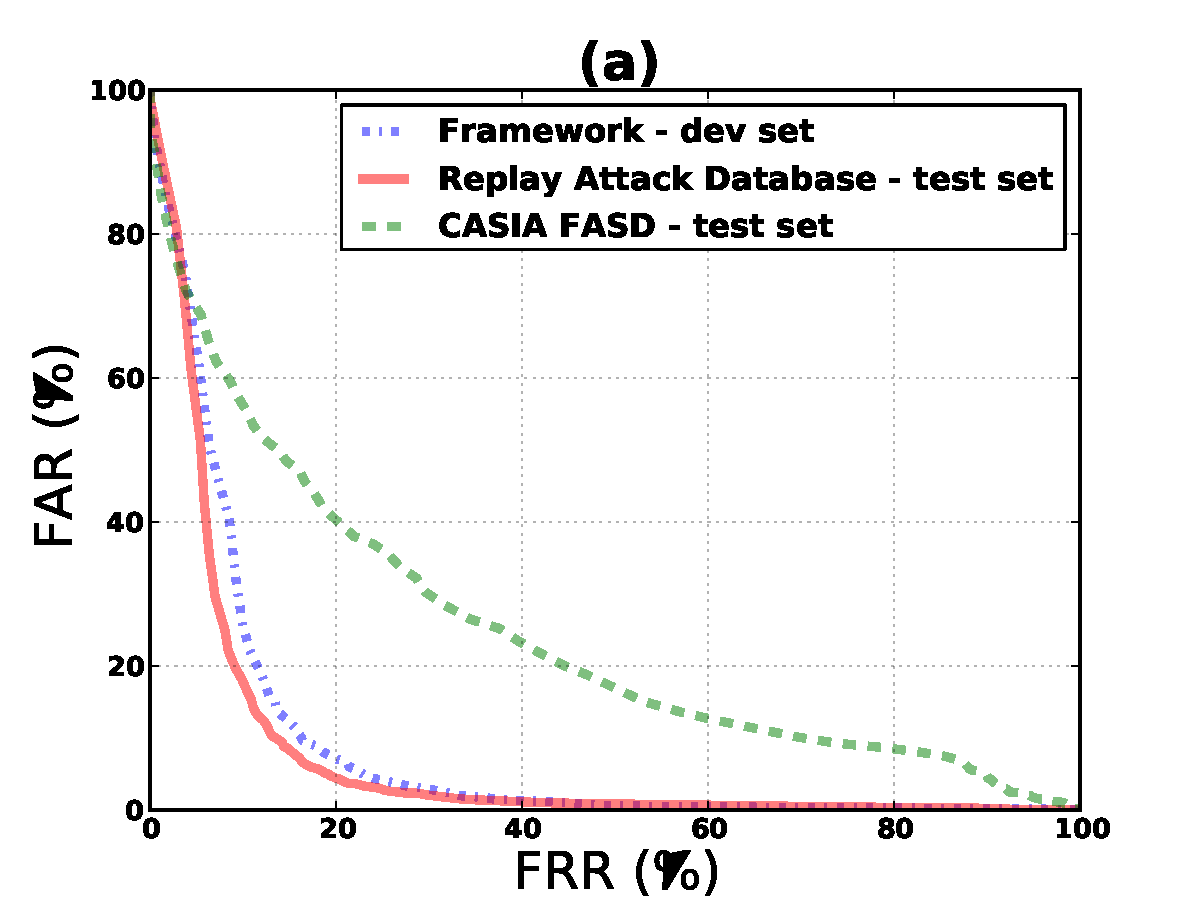
\includegraphics [width=5.5cm] {plots/FRAMEWORK/MOTION/SUM.pdf} 
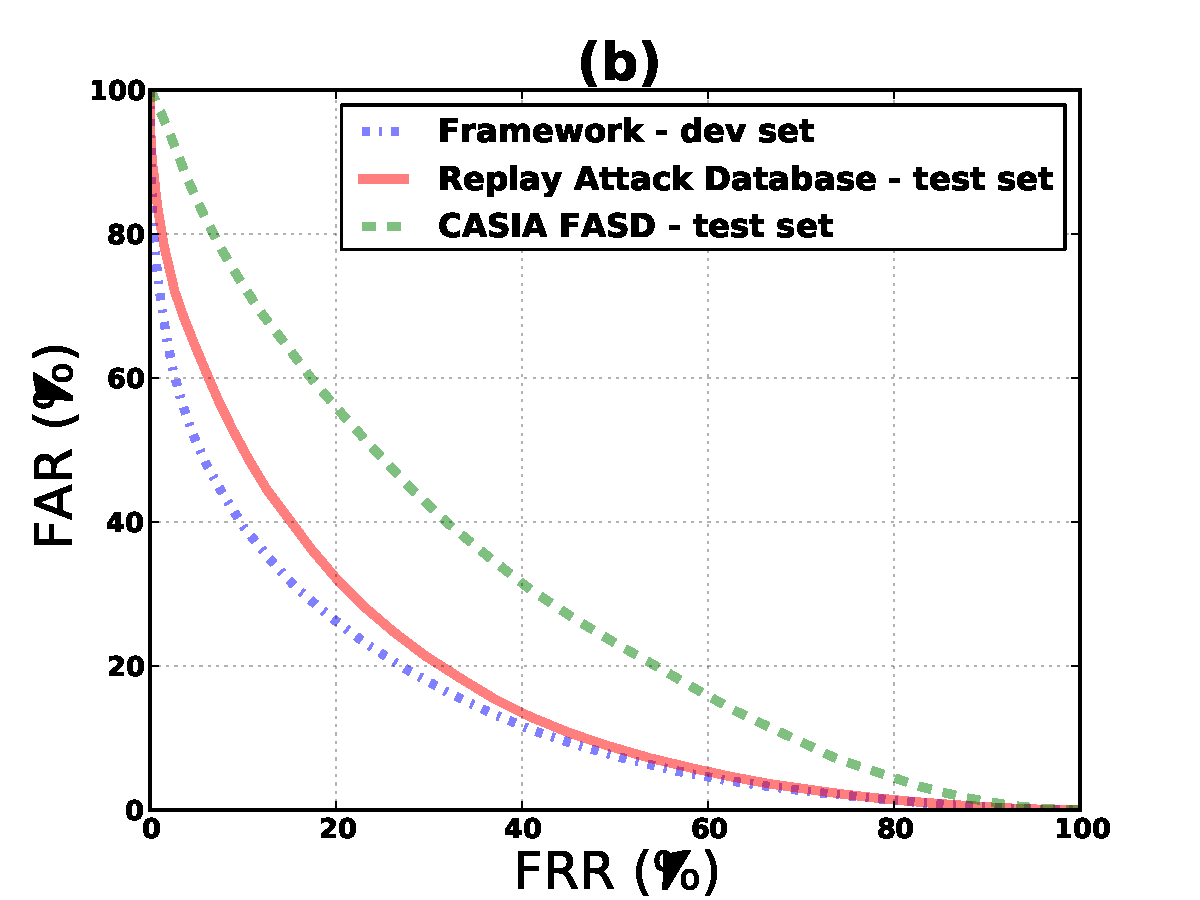
\includegraphics [width=5.5cm] {plots/FRAMEWORK/LBPTOP/SUM.pdf}
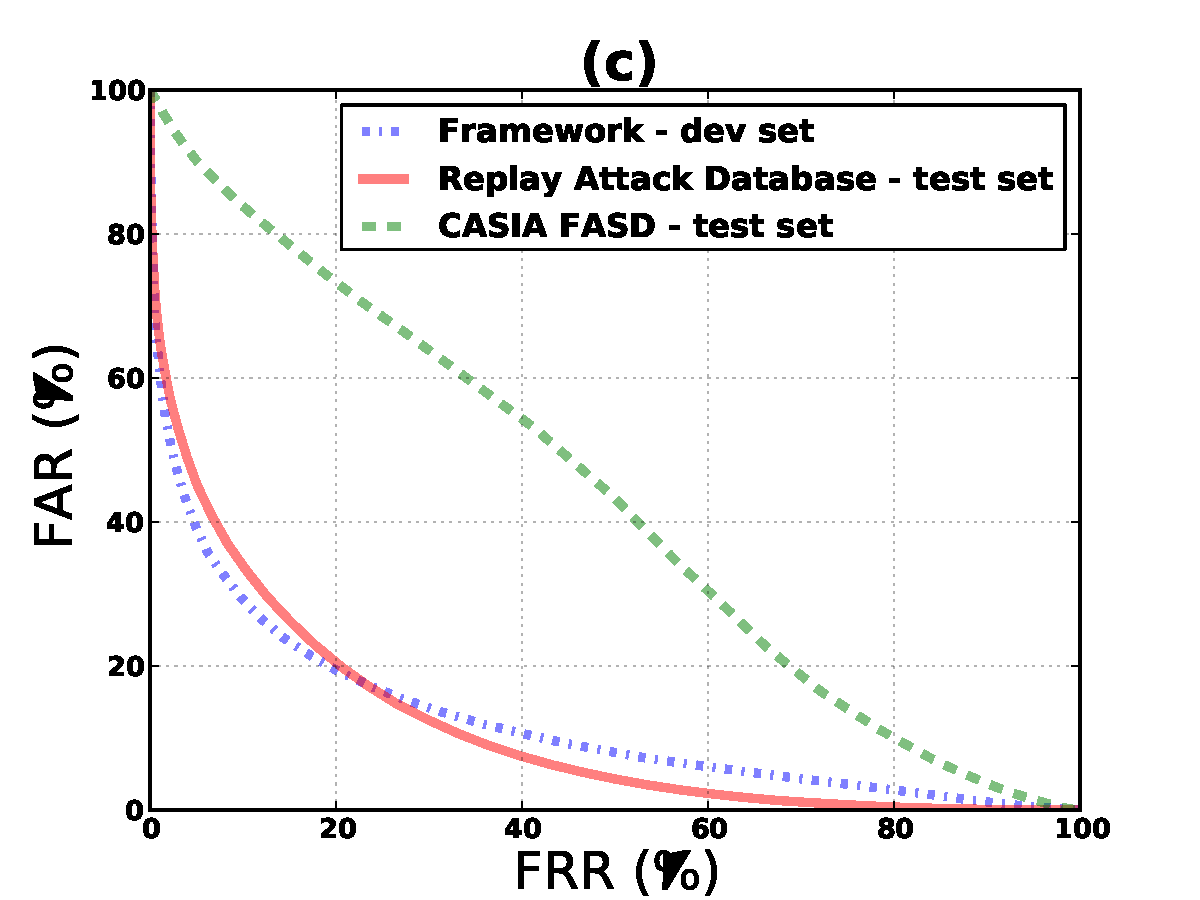
\includegraphics [width=5.5cm] {plots/FRAMEWORK/LBP/SUM.pdf}

\caption{ROC curves of each countermeasure trained with the Score Level Fusion based Framework (a) Correlation with frame differences (b) $LBP-TOP$ countermeasure (c) $LBP$ countermeasure.} 
\label{fig:ROC_framework}
\end{center}
\end{figure*}

Analyzing the $Q-statistic$ it is  possible to observe that the Correlation with Frame Differences countermeasure is the most statistically independent and suggests that a score fusion is suitable. This can be attested analysing its performance compared with the inter-test and intra-test protocol results (see Table \ref{tb:CrossTest}). For the inter-test protocol the improvement with the Score Level Fusion based Framework was significative ($\sim61.2\%$ in HTER average improvement). Comparing with the intra-test protocol the degradation was very low ($\sim3.6\%$ in HTER average) and the countermeasure is able to detect spoofs in both databases with different degrees of sucess.

However the $Q-statistic$ for the $LBP-TOP$ and the $LBP$ countermeasures present unbalanced values for each database. Specially for the CASIA FASD $Q_{R,C}\simeq-0.4$ suggesting that each one of this two countermeasure trained with different databases oppose each other and are not suitable for the Score Level Fusion based Framework. This can be attested analysing their performances compared with the intra-test protocol results (see Table \ref{tb:CrossTest}). The degradation is still high ($\sim106.7\%$ in $HTER(\%)$ average).

The authors that designed the $LBP$ and $LBP-TOP$ countermeasures chosen the SVM with the RBF kernel as classifier. In both settings, the final trained machines have $\sim35\%$ of the training data as support vectors, what suggest overfitting in each database. The authors that designed the Correlation with Frame Differences countermeasure chosen MLPs with only 5 neurons, which is much simpler classifier and has less chance to overfit of the training data than a SVM.

It is important to remark that the literature lacks in video face spoofing databases and is not possible to ensure the effectiveness of the Score Level Fusion based Framework in a third database. Its effectiveness in a third video face spoofing database, at this stage is only speculative. Another point to highlight is that the fusion strategy chosen for this work is quite simple. For a future extensions more complex fusion strategies need to be addressed.


\chapter{Conclusions}
\label{chap:Conclusions}

The goal of this masters dissertation was two fold. Firstly, we introduced a novel method to detect face spoofing using dynamic textures. The key idea of the method was to analyse the structure and the dynamics of micro-textures in the facial regions using the $LBP-TOP$ texture descriptor. The $LBP-TOP$ provides an efficient representation for the countermeasure. The experiments carried out with this countermeasure consistently outperform prior works on the Replay Attack Database and in the CASIA FASD (following their provided protocols). Best results were achieved using nonlinear SVM classifier, but it is important to notice that experiments with simpler LDA based classification scheme resulted in comparable performance under various spoofing attack scenarios. The use of simple and computationally efficient classifiers should be considered when constructing real-world anti-spoofing solutions.

Secondly, we compared four countermeasures, representative of the state of the art of this field, using two different test protocols. Using the two video face antispoofing databases publicly available (Replay Attack Database and CASIA FASD) we introduced the intra-test protocol and the inter-test protocol. The intra-test protocol enabled us to measure the performance and evaluate the intra-database generalization of countermeasures. The evaluation of each countermeasure using this protocol suggests that they are effective to detect spoofs in both databases. Even presenting different performances for different databases, the evaluated countermeasures presented a generalization capability. The only exception was the countermeasures based on eye blinks. With one eye blink, as a liveness check, this countermeasure was easy to deceive, with a $FAR$ higher than 90\%. Increasing the number of eye blinks the $FRR$ was higher than 90\%. The inter-test protocol enabled us to evaluate the inter-database generalization of the countermeasures. Using this protocol, it was observed that the evaluated countermeasures are sensitive to the databases biases. It was not possible to detect attacks from one database training the countermeasures with another database. It was observed two kinds of database bias. The first one, called \textbf{capture bias}, is a bias related to process of the databases construction. Both databases present different ways to carry out the attacks. The second one, called \textbf{attack bias}, is a bias related to the attacks. There are some attacks exclusive to the CASIA FASD and there are some exclusive to the Replay Attack Database.

In order to overcame these biases we introduce two approaches. The first one, combination of multiple databases, combines the train set of each database to train each one of the presented countermeasures. This strategy brought improvements, in HTER terms, compared with the inter-test protocol, but it was observed a strong bias to the Replay Attack Database. In the second approach, we introduced the Score Level Fusion based Framework that merges the scores of countermeasures trained with different databases. The results obtained with the Score Level Fusion based Framework suggest that combining two good and not correlated countermeasures leads to significant improvement in performance, in HTER terms, compared with both protocols. However, the literature lacks in video face spoofing databases; there are only two freely available. The effectiveness of the Score Level Fusion based Framework in a third video face spoofing database, at this stage is only speculative

\section{Contributions}

This masters dissertation provided the following contributions:

\begin{enumerate}
	\item An effective countermeasure against face spoofing attempts based on dynamic texture; 
	\item A comparative study on the state of the art countermeasures considering different databases and analysing possible biases that these databases can introduce in the countermeasures;
	\item A reproducible research. All source codes of this masters dissertation are freely available for download for future studies;
	%\item A method inspired in an antivirus to combine different countermeasures.
\end{enumerate}


\section{Future work}

As future work, we can suggest:

\begin{enumerate}
	\item Explore different $LBP$ operators in the $LBP-TOP$ planes;
	\item Construction of new face antispoofing database in order to measure the effectiveness of the Score Level Fusion based Framework;
	\item Evaluate different fusion strategies in the Score Level Fusion based Framework;
	\item Evaluate different organizations for the Score Level Fusion based Framework. For example, it is possible to cover ``micro" countermeasures, each one specialized in one type of attack. It is possible also to aggregate into the framework countermeasures that are complementary as in \citep{Komulainen_ICB_2013} or even consider the scores of a face verification as an element of the framework as in \citep{Chingovska_CVPRWORKSHOPONBIOMETRICS_2013}.

\end{enumerate}

%\appendix{Related Publications}
\begin{appendices}
\chapter{Texture Description with Local Binary Patterns}
\label{AppendixA}

The Local Binary Pattern (LBP) texture descriptor \cite{ojala1996comparative}, is computed in a pixel level basis using a $n \times n$ kernel, thresholding the surroundings of each pixel with the central pixel value and considering the result as a binary value. The decimal form of the LBP code is expressed as:

\begin{equation}
LBP(x_{c},y_{c})=\displaystyle\sum\limits_{n=0}^{N-1} \emph{f}(i_{n}-i_{c})2^n,
\label{eq:LBP}
\end{equation}

\noindent where $i_{c}$ corresponds to the gray intensity of the center pixel ($x_{c}, y_{c}$), $N$ is the number of sampling points, $i_{n}$ is the gray intensity of the n-th surrounding pixel, and $f(x)$ is defined as follows:

\begin{equation}
f(x)  =
\left\lbrace \begin{array}{ccc}
0 & \mbox{if} & x<0 \\
1 & \mbox{if} & x\geq0 
\end{array}. \right.
\label{eq:fx}
\end{equation}

Later, Ojala et al. \cite{ojala2002multiresolution} extended this operator to support surrounding points and radius of a pixel neighbourhood with different shapes and sizes, enabling handling textures at different scales. Fig. \ref{fig_lbpOperator} illustrates the operator calculation and the points distribution in a circular neighbourhood with radius 2, where the pixel values are bilinearly interpolated whenever the sampling point is not in the center of a pixel.

\begin{figure}
\begin{center}
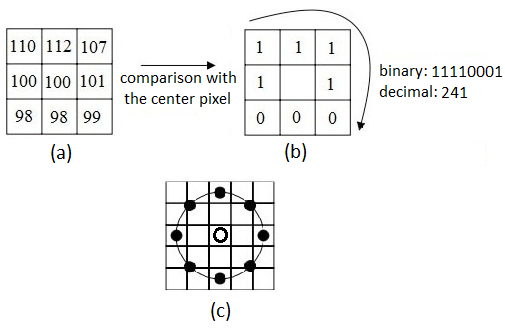
\includegraphics [width=7.5cm] {images/lbp_operator}
\caption{LBP operator. (a) and (b) The basic LBP operator, where the neighbourhood of each pixel is thresholded and a binary number is obtained. (c) A circular neighbourhood example (with 8 neighbour points and radius 2). The pixel values are bilinearly interpolated whenever the sampling point is not in the center of a pixel.} \label{fig_lbpOperator}
\end{center}
\end{figure}

Another important extension proposed by Ojala et al. \cite{ojala2002multiresolution} was the uniform patterns concept ($u2$). A LBP operator is considered uniform if it contains at most two bitwise transitions 0-1 or 1-0 when viewed as a circular bits chain, and according to Ojala et al. \cite{ojala2002multiresolution}, nearly 90 percent of LBP operators observed in images are uniform. In spacial terms, uniform patterns represent some patterns of a texture: spot, flat, area, edge and corner. With an 8-bit representation, there are 58 patterns with at most two bitwise transitions. Fig. \ref{fig_uniformPattern}, extracted from \cite{Chan2008}, describes all possible uniform patterns with 8 neighbours.

\begin{figure}
\begin{center}
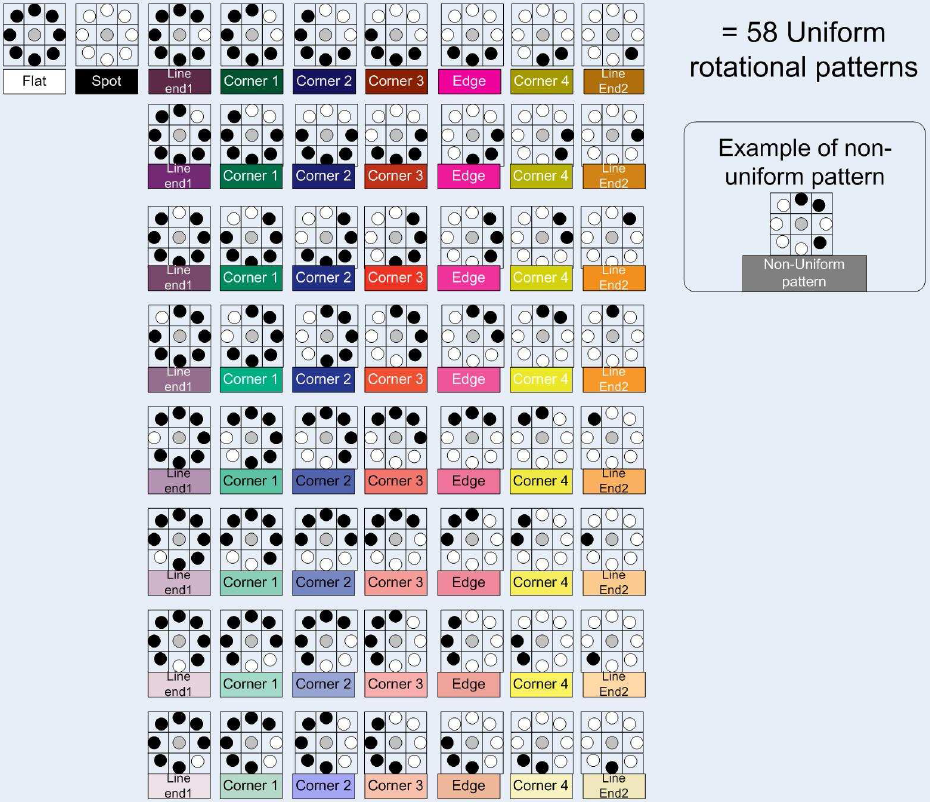
\includegraphics [width=12cm] {images/fig_uniformPattern} 
\end{center}
   \caption[All uniform patterns for LBP with 8 neighbours]{All uniform patterns for LBP with 8 neighbours \cite{Chan2008}.}   
\label{fig_uniformPattern}
\end{figure}

Ahonen et al. (see \cite{ahonen2004face} and \cite{ahonen2006face}) adopt the following notation for the LBP operator: $LBP_{P,R}^{u2}$, where the subscript represents the neighbourhood configuration with $P$ sampling points on a circle of radius $R$, and the superscript $u2$ stands for using only uniform patterns and labelling all non-uniform patterns with a single label.

Recently, LBP have been applied to represent face images, yielding in promising results \cite{ahonen2004face}. The face description using LBP consists in computing a histogram of LBP operators, and good results have been achieved using a configuration with 8 circular surrounding pixels and radius 2 (see \cite{ahonen2004face}, \cite{ahonen2006face} and \cite{Rodriguez06}). The LBP histogram-based approach for face description also takes advantage of the LBP operator extensions. As an example, when uniform patterns are used, the number of histogram bins is greatly reduced, since all non-uniform patterns are grouped into a single bin.

A relevant modification in the original LBP operator for face representation is the idea of splitting the face image in small blocks (which can be overlapped or not) and computing the LBP histogram for each block individually, thereby retaining spatial information. So, the face image is described in three different levels: a pixel level, with the calculation of each operator individually; the regional level, with the calculation of histograms for each block; and a global level, with the concatenation of all block histograms \cite{Rodriguez06}. Fig. \ref{fig_lbpDescription} shows all three levels of face description.


\chapter{Related Publications}
\label{AppendixB}


\end{appendices}


%=============================== Bibliografia ===============================================
\addcontentsline{toc}{chapter}{References}
\renewcommand{\bibname}{References}
\markboth{References}{References}

\bibliographystyle{dcu}
\bibliography{meubib}


\end{document}
